\chapter{Homogeneous Boltzmann equation: sparse Fourier spectral scheme}
\chaptermark{HBE: sparse Fourier spectral scheme}
\label{chap:boltzmann-fourier}

\section{Introduction} 
\label{sect:boltzmann}

For the remainder of this dissertation, we will focus on the spatially homogeneous Boltzmann equation,
\begin{equation} \label{eqn:boltzmann-sphom}
    \frac{\partial f}{\partial t} = Q(f,f),
\end{equation}
where $Q$ is the Boltzmann collision operator introduced in Section~\ref{sec:boltzmann-intro}.

The most popular methods for the solution of \eqref{eqn:boltzmann-sphom} are stochastic Monte Carlo-type
methods. Determenistic schemes do not suffer from problems of indeterminism, noise and slow convergence, but
they are generally very expensive. Lattice Boltzmann methods, which rely on very crude pointwise
discretizations in velocity space have also become popular. Since our work is primarily concerned with
high-accuracy spectral determenistic methods, no attempt will be made in the following to compare our work
with stochastic methods or lattice Boltzmann methods.

Existing work on the discretization of \eqref{eqn:boltzmann-sphom} rely heavily on Fourier spectral
discretization, which can exploit the convolution structure of $Q$ owing to the translation invariance of
Theorem~\ref{thm:trans-rot-Q}. See
\cite{Bobylev1988tns, Kirsch2007wfb, Pareschi1996fsm} and
\cite{Gamba2009slm, Gamba2010sbs, Filbet2006sbe, Pareschi2000nsb, Pareschi2003smb}
for numerical simulations based on that method. Also related to this are the
difference methods developed in
\cite{Bobylev1997dsb, Bobylev1999fdm, Bobylev2000nsb} and \cite{Ibragimov2002nsb}.

The approach entails two fundamental modifications of the collision operator:
\begin{enumerate}
  \renewcommand{\labelenumi}{(\roman{enumi})}
  \item the restriction of the integration over $\bbR^{d}$ in~(\ref{eqn:Q-std}) to 
    a ball of finite radius $R>0$, see Section~\ref{sec:trunc} for details, 
  \item the truncation of the velocity space $\bbR^{d}$ to a cube $\cD_{L} := [-L,L)^{d}$ plus
    periodic continuation. 
\end{enumerate}
These result in a perturbed evolution
\begin{gather}
  \label{eqn:QR}
  \frac{\partial}{\partial t}{f}_R = Q^R(f_R, f_R), \qquad f(0) = f_0.
\end{gather}
Clearly, its solution depends on both $R$ and $L$. The exact definition of $Q^R$ will be given in
Section~\ref{sec:fourier}.

Subsequently, \eqref{eqn:QR} is projected onto a subspace of $L^{2}(\cD_{L})$ spanned by a
finite set of Fourier modes. An in-depth analysis of the discretization error due
to this last step has recently been developed by Filbet and Mouhot in \cite{Filbet2011asm},
and in parts of our work we are going to rely on their techniques. 

One of our main goals was to provide a priori estimates of the discretization error for \eqref{eqn:QR} in
$H^{s}$-Sobolev norms, $s\geq 0$, for rather general sets of Fourier modes, which includes as a special cases
the so-called hyperbolic crosses. For certain types of solutions, this scheme offers much more efficient
approximation compared to the full tensor product space of Fourier modes. This extends the results of
\cite{Filbet2011asm}.

In another respect we go beyond \cite{Filbet2011asm}: we also quantify the impact of
switching from (\ref{eqn:boltzmann-sphom}) to (\ref{eqn:QR}), conditional
on the following conjecture.
\begin{conjecture} \label{ass:decay}
  For given Sobolev index $s\geq 0$, assume that there exist $C_0>0$ and $a>0$ so that the solution
  $f_R$ of \eqref{eqn:QR} fulfills
  $$
  |\partial^\Balpha f_R(t,\Bv)| \le C_0\exp\left(-a|\Bv|^2\right),
  $$
  and that there exists a polynomial $\Pi(L)$ so that
  $$
  \| \exp\left(a|\Bv|^2\right) \partial^\Balpha f_R(t,\Bv) \|_{L^2(\cD_L)} \leq
  \Pi(L),
  $$
  for all $|\Balpha|_1\leq s$, $t\geq0$ and $f_{R}$ solving (\ref{eqn:QR}).
\end{conjecture}
\begin{remark}
  The decay condition on $f_R$ is formulated in this form since it is
  $2L$-periodic, and thus it cannot satisfy any classical decay condition on the
  whole of $\bbR^d$. The polynomial dependence on $L$ is allowed so that 
  equilibrium solutions fit the assumption. For example, if $\Balpha=0$ and 
  $f_R(t,\Bv)=\exp(-a|\Bv|^2)$ we require $\Pi(L) \geq (2L)^{\nicefrac{d}{2}}$.
  
  The decay of $f$ is well known, see for example \cite{Bobylev1997mib}.  Yet, so far,
  there is no rigorous proof that the Conjecture~\ref{ass:decay} holds for
  $f_R$. We have only numerical evidence that this is true, see
  Section~\ref{sec:decay}.
\end{remark}

\textbf{Outline.} The chapter is structured as follows. In Section \ref{sec:fourier}
we develop the details of the truncation of $Q$ and the Fourier spectral discretization.
The following Section~\ref{sec:hyper} introduces the concrete Fourier spectral 
Galerkin discretization of (\ref{eqn:QR}) for families of hyperbolic cross Fourier
modes. In Section~\ref{sec:appr} we develop the main a priori convergence
estimates, which are summarized in Theorem~\ref{thm:mainapprox} (consistency
estimates), Theorem~\ref{thm:discrerror} (Fourier spectral discretization error
for (\ref{eqn:QR})), and Proposition~\ref{prop:err-R} (estimate for $f-f_{R}$). 
We emphasize that Conjecture~\ref{ass:decay} is essential only for this last result.

Numerical experiments for all Fourier-based methods discussed are reported in Section~\ref{sec:numerical-fou}.
They highlight the conditions that have to met for satisfactory performance of the hyperbolic cross
approximation.  They also convey the importance of choosing a sufficiently small ratio $R:L$ in order to avoid
aliasing.

\section[Fourier discretization of the Boltzmann collision operator]{Fourier discretization of the Boltzmann collision operator%
    \sectionmark{Fourier discr. of the Boltzmann collision operator}}
\sectionmark{Fourier discr. of the Boltzmann collision operator}
\label{sec:fourier}

In this section we aim to discretize the solution $f$ by a finite Fourier
series. Of course, integrals such as \eqref{eqn:Q-p} and \eqref{eqn:Q-m} will
diverge for periodic $f$. Thus, a truncation in velocity is required.

\subsection{Truncation in velocity space} \label{sec:trunc}

In this section, we develop equivalent {\em truncated} forms for the collision
operator as defined via
\begin{equation} \label{eqn:Q-p}
    Q(f,h)(\Bv) = \int_{\bbR^d}\int_{\bbS^{d-1}} B(|\Bg|,\cos\theta)(h_*'f' -
    h(\Bv-\Bg)f(\Bv))\dd\Bsigma \dd \Bg,
\end{equation}
which is achieved through a change of variables $\Bg=\Bv-\Bv_*$, and the {\em
Carleman representation}
\begin{multline} \label{eqn:Q-m}
    Q(f,h)(\Bv) = \int_{\bbR^d}\int_{\bbR^d} \Bt(\Bx,\By) \delta(\Bx\cdot\By) \\
    \left[ h(\Bv+\By)f(\Bv+\Bx) - h(\Bv+\Bx+\By)f(\Bv) \right] \dd \Bx \dd \By,
\end{multline}
whose derivation is detailed in \cite{Mouhot2006fac} and also in \cite{Bobylev1999fdm} for hard sphere collision
kernels ($B\equiv|\Bg|$).

The following proposition is given in \cite{Pareschi2000nsb}, with $\B_R$ denoting
the ball of radius $R$ centered at $0$. It follows more or less straightforwardly from \cite{Pareschi1996fsm}.
\begin{proposition}[Proposition 3.1 in \cite{Pareschi2000nsb}] \label{prop:trunc}
Let $\supp f,h\subseteq\B_R$. Then, $\supp Q(f,h)\subseteq\Bsr$, and 
\[ 
    Q(f,h)(\Bv) = \int_{\Btr}\int_{\bbS^{d-1}} 
            B(|\Bg|,\cos\theta)(h_*'f'-h_*f)\dd\Bsigma \dd \Bg 
\]
for $\Bv\in\Bsr$. Under these assumptions,
$\Bv',\Bv_*',\Bv-\Bg\in\B_{(2+\sqrt{2})R}$ for all $\Bg\in\Btr$.
\end{proposition}
Thus, by considering $f$ restricted on the cube $\cD_L=[-L,L]^d$, with
$f(\Bv)=0$ on $\cD_L\setminus\B_R$, extended periodically to all of $\bbR^d$, we
can evaluate $Q(f,f)$ without aliasing if $\nicefrac{R}{L}$ is small enough. In
practice, $L$ should be chosen large enough to accommodate the necessary number
of timesteps while minimizing the aliasing errors, as the support of $f$ will
grow.

Common practice \cite{Pareschi2000nsb, Mouhot2006fac} is to choose $R,L$ so that aliasing is avoided for one
single application of the collision operator. This holds if
$$
    \kappa = \frac{R}{L} \leq \frac{2}{3+\sqrt{2}},
$$
see for example \cite[Fig. 1]{Pareschi2000nsb}.  In Section~\ref{sec:aliasing} we present some numerical
experiments showing how the choice of $\kappa$ can significantly impact the performance of a numerical scheme.

The task is now to bring the Carleman representation \eqref{eqn:Q-m} into
truncated form also, so that the two truncated representations are equivalent.
This is the content of the following proposition.

\begin{proposition} \label{prop:equiv}
Consider $f$ and $h$ restricted to the cube $\cD_L$ with $f(\Bv)=0$ on
$\cD_L\setminus\B_R$, extended periodically to all of $\bbR^d$, with
$\kappa=\nicefrac{R}{L}\leq\nicefrac{2}{(3+\sqrt{2})}$. Then, for $v\in\Bsr$, the
following representations of $Q(f,h)(\Bv)$ agree.
\begin{align}
    \label{eqn:Q-p-b}
    Q^R_{\mathrm{P}}(f,h) &\defeq 
    \int_{\Btr}\int_{\bbS^{d-1}} B(|\Bg|,\theta)(h_*'f'-h_*f)\dd\Bsigma \dd \Bg \\
    \label{eqn:Q-m-b} 
    Q^R_{\mathrm{M}}(f,h) &\defeq \int_{\Bsr}\int_{\Bsr} \Bt(\Bx,\By)\delta(\Bx\cdot \By) \\
    \nonumber & \qquad\qquad\qquad\qquad
        \left[ h(\Bv+\By)f(\Bv+\Bx) - h(\Bv+\Bx+\By)f(\Bv) \right] \dd \Bx \dd \By
\end{align}
\end{proposition}
\begin{proof}
Representation \eqref{eqn:Q-p-b} follows from Proposition \ref{prop:trunc}.
Following the policy from \cite{Mouhot2006fac}, it can be shown that
\begin{multline*}
    Q(f,h)(\Bv) = \int_{\bbR^d}\int_{\bbR^d}\Bt(\Bx,\By)\delta(\Bx\cdot \By)\chi_{\B_{2R}}(\Bx+\By)  \\ 
    \left[h(\Bv+\By)f(\Bv+\Bx)-h(\Bv+\Bx+\By)f(\Bv)\right] \dd \Bx \dd \By. 
\end{multline*}
It remains to show that when $|\Bx+\By|>2R$, i.e. when
$\chi_{\Btr}(\Bx+\By)=0$, we have $h(\Bv+\By)f(\Bv+\Bx) = h(\Bv+\Bx+\By)f(\Bv)
= 0$.

Under these assumptions, it is clear that either $|\Bv|>R$ or
$|\Bv+\Bx+\By|>R$. Furthermore, since $\Bx\perp \By$, we also have
$|\Bx-\By|>2R$, so either $|\Bv+\By|>R$ or $|\Bv+\Bx| =
|(\Bv+\By)+(\Bx-\By)| > R$.

Last, for $|\Bx|,|\By|\leq\sqrt{2}R$, we have
\[
    \max\{|\Bv|,|\Bv+\Bx|,|\Bv+\By|,|\Bv+\Bx+\By|\} \leq 2L-R,
\]
so aliasing is avoided. This concludes the proof.
\end{proof}

Henceforth, we will denote by $Q^R$ the truncated version of $Q$ as defined in \eqref{eqn:Q-p-b} and
\eqref{eqn:Q-m-b}. We will also denote by $Q^{R,+}$ and $Q^{R,-}$ the corresponding truncated versions of
$Q^+$ and $Q^-$. We will always assume that the ratio of $R$ and $L$ is fixed and denote it by the constant
truncation parameter $\kappa=\nicefrac{R}{L}$.

\subsection{Fourier discretization} \label{sec:FourierDiscretization}

Following ideas from \cite{Gottlieb1977nas, Canuto1988smf}, let us now discretize $f$ by
representing it as a truncated $d$-dimensional Fourier series in $\Bv$, 
\begin{equation} \label{eqn:fn}
    f_\cA(t,\Bv) = \sum_{\Bk\in\cA} \hf_\Bk(t) \ee^{\ii\Bk\cdot\Bv},
\end{equation}
where $\cA\subset(\nicefrac{\pi}{L})\bbZ^d$ is some discrete and finite but so far
unspecified set of Fourier modes. Then, \eqref{eqn:boltzmann-sphom} yields
\begin{equation} \label{eqn:boltzmann-d-1}
    \sum_{\Bk\in\cA} \frac{\dd \hf_\Bk}{\dd t} \ee^{\ii\Bk\cdot \Bv} = \sum_{\Bl,\Bm\in\cA}
            \hf_\Bl\hf_\Bm Q^R\left(\ee^{\ii\Bl\cdot \Bv},
            \ee^{\ii\Bm\cdot \Bv}\right).
\end{equation}
Substituting the Fourier modes into \eqref{eqn:Q-p} or \eqref{eqn:Q-m}, we find
that there exist coefficients $\hbeta(\Bl,\Bm)$ so that
\begin{equation} \label{eqn:kmodes}
    Q^R\left(\ee^{\ii\Bl\cdot \Bv},\ee^{\ii\Bm\cdot \Bv}\right) = 
            \hbeta(\Bl,\Bm)\ee^{\ii(\Bm+\Bl)\cdot \Bv}
\end{equation}
for all $\Bl,\Bm \in (\nicefrac{\pi}{L})\bbZ^d$. This follows easily from a straightforward generalization of
Theorem~\ref{thm:trans-rot-Q}, since the transformation $\Bv \mapsto \Bv-\Bc$ leaves $\Bg$ and $\Bsigma$
unchanged. Equation \eqref{eqn:kmodes} is in many ways {\em raison d'\^{e}tre} for the whole method---the
justification for our transgressions in truncating $Q$.

Plugging this into \eqref{eqn:boltzmann-d-1}, discarding coefficients outside
$\cA$ and comparing the remaining coefficients, gives us the following quadratic
ordinary differential equation (ODE) for the coefficients $\hf_\Bk$:
\begin{equation} \label{eqn:boltzmann-d}
    \frac{\dd \hf_\Bk}{\dd t} = \sum_{\substack{\Bl,\Bm\in\cA \\
    \Bl+\Bm=\Bk}} \hf_\Bl\hf_\Bm\hbeta(\Bl,\Bm),\quad \Bk\in \cA.
\end{equation}
This is the Fourier space equivalent to seeking $f_\cA \in \spann \{ \ee^{\ii\Bl\cdot\Bv} \;:\; \Bl\in\cA \}$
so that
\begin{equation} \label{eqn:boltzmann-nd}
  \frac{\partial}{\partial t} {f}_\cA = P_\cA Q^R(f_\cA,f_\cA)
\end{equation}
where $P_\cA$ is the $L^2$-orthogonal projection on the the space spanned by the Fourier modes in $\cA$.

The coefficients $\hbeta(\Bl,\Bm)$ are called the {\em kernel modes}. These can be
evaluated through \eqref{eqn:kmodes}.  Note that since the Fourier modes
$\ee^{\ii\Bk\cdot \Bv}$ do not satisfy the conditions of Proposition
\ref{prop:equiv}, representations \eqref{eqn:Q-p-b} and \eqref{eqn:Q-m-b} will
yield {\em different} values for $\hbeta$. In the following, we will denote by
$\hbeta_d^\rmP$ those values arising from \eqref{eqn:Q-p-b}, and by $\hbeta_d^\rmM$ those
arising from \eqref{eqn:Q-m-b}. 

Separating gain and loss terms as described in Section~\ref{sect:boltzmann}, we
find that we have 
\[ 
    \hbeta_d^\ast(\Bl,\Bm) = \beta_d^\ast(\Bl,\Bm) - \beta_d^\ast(\Bm,\Bm),\qquad
    \ast \in \{\rmP,\rmM\}
\]
where the coefficients $\beta_d^\ast$ are given, for general kernels $B$ and $\Bt$, as 
\begin{multline} \label{eqn:B-p} 
    \beta_d^\rmP(\Bl,\Bm) = \int_{\Btr}\int_{\bbS^{d-1}} B(|\Bg|,\cos\theta) \\
    \exp\left[ -\ii\Bg\cdot\frac{\Bl+\Bm}{2} - 
        \ii|\Bg|\Bsigma\cdot\frac{\Bm-\Bl}{2} \right] \dd\Bsigma \dd \Bg
\end{multline}
and
\begin{equation} \label{eqn:B-m} 
    \beta_d^\rmM(\Bl,\Bm) = \int_{\Bsr}\int_{\Bsr} 
        \Bt(\Bx,\By)\delta(\Bx\cdot \By) \ee^{\ii\Bl\cdot \Bx} 
        \ee^{\ii\Bm\cdot \By} \dd \Bx \dd \By,
\end{equation}
for $\Bl,\Bm\in\cA$. For more information regarding efficient computation of kernel modes we refer to
\cite{Pareschi2000nsb,Mouhot2006fac}.

\section{Choice of $\cA$} \label{sec:hyper}

So far, we have left the choice of Fourier space $\cA$ unaccounted for. Of
course, it is required that $\cA$ is a subset of the scaled lattice grid
\[ 
    \cA \subset \frac{\pi}{L}\bbZ^d. 
\]
The obvious choice, and the one adopted in \cite{Pareschi2000nsb} and
\cite{Mouhot2006fac} is the full $d$-dimensional discrete Fourier
representation with $N$ degrees of freedom in each direction:
\[
    \AFF(N) = \frac{\pi}{L}\left\{-\frac{N}{2}, -\frac{N}{2}+1, \ldots, 
            \frac{N}{2}-1\right\}^d.
\]

An alternative choice is the {\em hyperbolic cross} Fourier space, which can be
considered the frequency-space equivalent of sparse grids (see for example
\cite{Gradinaru2007fts,Knapek2000hca,Griebel2013fdf} for more details),
\[
    \cA_Y(N):= \left\{ \Bk\in \frac{\pi}{L}\bbZ^d \;:\; \prod_{j=1}^d(1+|\tilde{k}_j|)
            \cdot (1+|\tilde{\Bk}|_\infty)^{-Y} \le (1+N)^{1-Y} \right\},
\]
where $Y\leq1$, with the limiting set $A_{-\infty}(N) = \AFF(N)$, and where the
vectors $\Bk$ and $\tilde{\Bk}$ are related by
\[
    \Bk = \frac{\pi}{L}\tilde{\Bk},
\]
rendering $\tilde{\Bk}$ integral. 

Thus, we deal with two discretization parameters: (i) the parameter $Y$, which controls the ``fatness'' of the
hyperbolic cross, with the classical hyperbolic cross being given by $Y=0$, and (ii) the ``resolution
parameter'' $N$.  For $Y=0$, we have $\sharp\cA_0(N)=\cO(N(\log N)^d)$ compared to $\sharp\AFF(N)=N^d$.

Importantly, the hyperbolic cross does {\em not} provide good approximations of near-Maxwellians. Indeed, the
spectrum of a Maxwellian is a Maxwellian centered at the origin, and its rotational symmetry makes it well
suited for an approximation by $\AFF(N)$, see Figure~\ref{fig:hcgauss}.

\begin{figure}
    \centering
    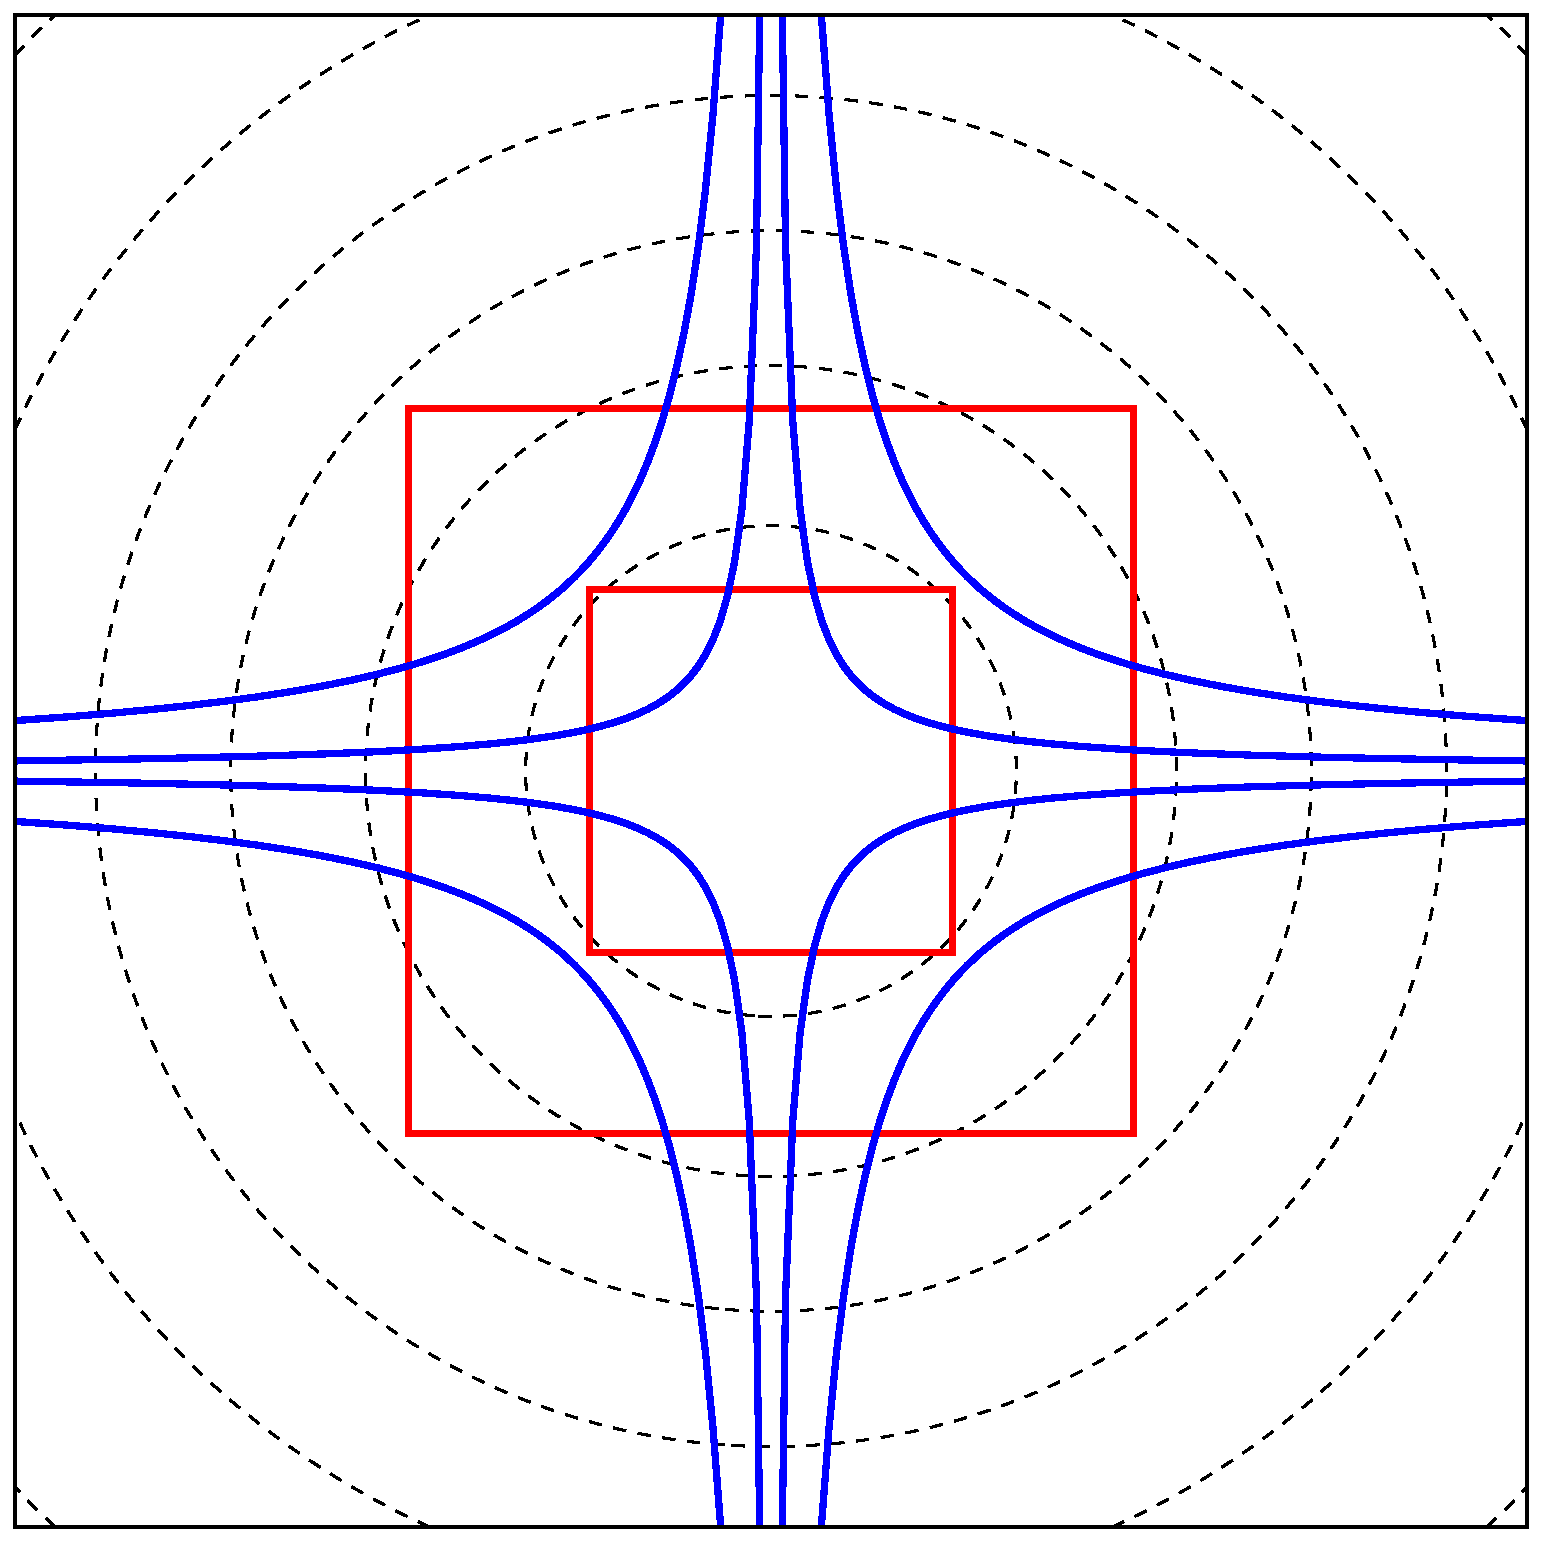
\includegraphics[width=6cm]{figs/hcboltz/hcgauss}
    \caption{Contour plot of the amplitude of the spectrum of a Gaussian, with the
             Fourier modes belonging to hyperbolic crosses and full grids of
             comparable size delineated for comparison. It seems that full
             grids offer much better approximation of Gaussians.}
    \label{fig:hcgauss}
\end{figure}

This indicates that the hyperbolic cross would be a poor choice for approximating
near-equilibrium solutions.  Of course, it could still provide a useful tool for
certain situations with $f$ far removed from equilibrium.  Moreover, the results
in this paper are not confined to the classical hyperbolic cross ($Y=0$) but to
the whole family of sampling sets $\cA_Y$, as well as $\AFF$, which allows
fine-tuning according to the degree of isotropy in the solution.

\subsection{Observables}

For the linear functionals mass density ($\rho$), momentum ($\Bu$) and energy ($E$), which define the
equilibrium solution, we have representations in terms of the coefficients $\hf_\Bk$ from \eqref{eqn:fn}:
\begin{gather*}
    \rho(f) = \frac{1}{(2L)^d}\sum_{\Bk\in\cA} \hat{\rho}_\Bk\hf_\Bk, \quad
    (\rho\Bu)(f) = \frac{1}{(2L)^d}\sum_{\Bk\in\cA} \hat{\Bu}_\Bk\hf_\Bk\\
    (\rho E)(f) = \frac{1}{(2L)^d}\sum_{\Bk\in\cA} \hat{E}_\Bk\hf_\Bk.
\end{gather*}
The quantities $\hat{\rho}_\Bk$, $\hat{\Bu}_\Bk$ and $\hat{E}_\Bk$ are given as
(re-scaled) Fourier coefficients of the functions $1$, $\Bv$ and $|\Bv|^2$:
\[
    \frac{1}{(2L)^d}
    \begin{pmatrix} 
        \hat{\rho}_\Bk \\ \hat{\Bu}_\Bk \\ \hat{E}_\Bk 
    \end{pmatrix} 
    = \int_{\cD_L} 
    \begin{pmatrix} 
        1 \\ \Bv \\ |\Bv|^2 
    \end{pmatrix} 
    e^{i\Bk\cdot \Bv} \dd \Bv
\]

Clearly, for mass density, we have $\hat{\rho}_\Bk = (2L)^d\delta_{\Bk,\Bzero}$.

For $\Bu$ and $E$, we find that $\hat{\Bu}_\Bk = \hat{E}_\Bk = 0$ whenever
$\Bk$ is off the axes, i.e. there is more than one nonzero element of $\Bk$.
Thus, let $\Bk = \frac{\pi}{L}\tilde{k}_j\Be_j$, where $\Be_j$ is the $j$'th
Cartesian basis vector, and $\tilde{k}_j$ some integer. 

Then we obtain
\begin{align*}
    (\hat{\Bu}_\Bk)_l &= 
    \begin{cases} 
        -i\frac{(-1)^{\tilde{k}_j}}{k_j}, & l=j \quad\text{and}\quad 
                \Bk\neq\Bzero \\ 
        0, & l\neq j \quad\text{or}\quad \Bk = \Bzero. 
    \end{cases} \\
    \hat{E}_\Bk &= 
    \begin{cases} 
        2\frac{(-1)^{\tilde{k}_j}}{k_j^2}, & \Bk\neq\Bzero, \\
        \frac{d}{3}L^2, & \Bk = \Bzero.
    \end{cases}
\end{align*}

Thus we see that even if $\cA$ is relatively large, say a box of $N^d$ degrees
of freedom, the accurate evaluation of these functionals require only a subset
of $\cA$ containing the axes, which are of size $\cO(dN)$.

It's also worth noting that $\AFF(N) \supseteq \cA_Y(N)$, yet for any functional
$\ell$ that depends only on Fourier coefficients on the axes (such as $\rho$,
$\Bu$ and $E$), we have
\[
    \ell\left(P_{\cA_Y(N)}f\right) = \ell\left(P_{\AFF(N)}f\right).
\]
The full grid offers no advantage over $\cA_Y$ in terms of such functionals, although off-axis modes will of
course impact the on-axis modes during evolution.

\subsection{Cost of evaluating $P_\cA Q^R(f_\cA,f_\cA)$}

The evaluation of $Q(f_\cA,f_\cA)$ requires the formation of the sum \eqref{eqn:boltzmann-d}. There are no
fast algorithms to compute this, unless some kind of separability of $\hbeta$ is available, as in
\cite{Mouhot2006fac}, which seems to be the case only for certain specific kernels $B$. In these cases the sum has
a convolution structure and we can evaluate the collision operator by using an FFT method requiring log-linear
time ($\cO(dN\log(N))$, where $N$ is the number of degrees of freedom in one dimension).

Without this convolution structure, a straightforward naive implementation has cost proportional to the
cardinality of the combination set
\[
    c(\cA) = \left\{ (\Bl,\Bm)\in\cA^2 \;:\; \Bl+\Bm\in\cA \right\}.
\]
The worst possible case for any $\cA$ is $\sharp c(\cA(N)) \in \cO([\sharp \cA(N)]^2)$, and for the the full grid
this bound is sharp. However, the hyperbolic cross can do better. For $Y=0$, we have experimentally that
\[
    \sharp c(\cA_0(N)) \in \cO(\sharp\cA_0(N)^{\nicefrac{15}{8}}),
\]
see Figure \ref{fig:complexity}.

\begin{figure}
    \centering
    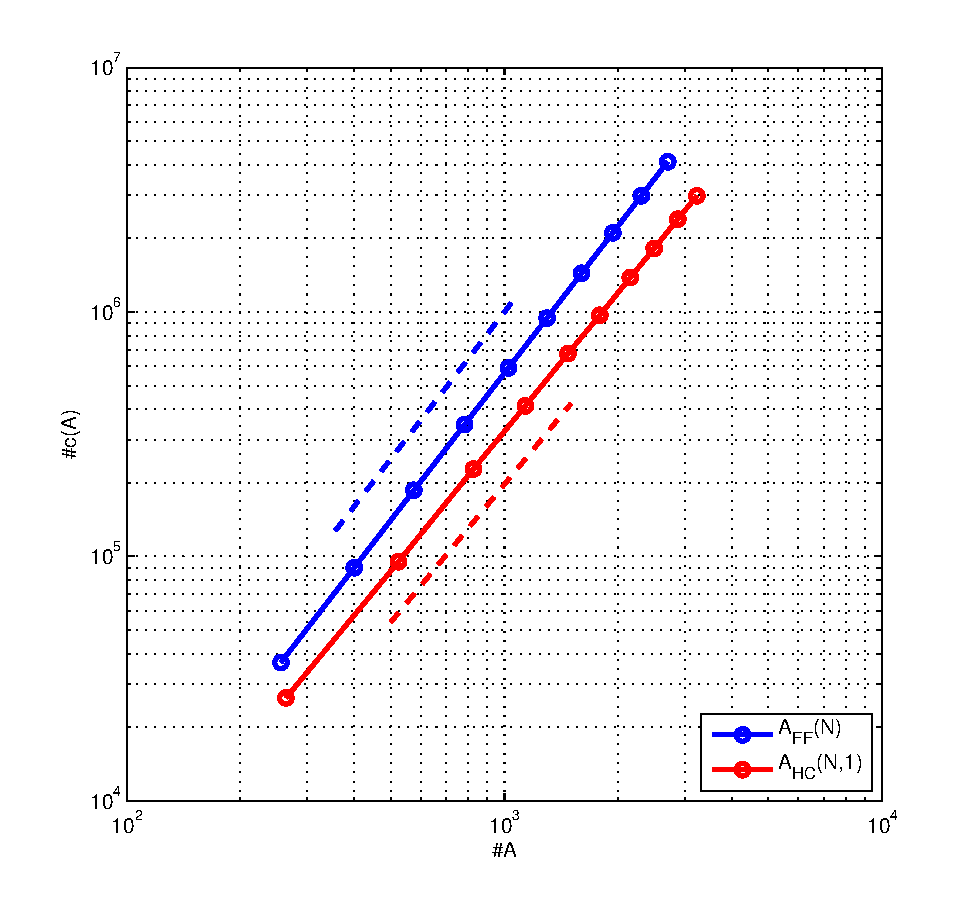
\includegraphics[width=12cm]{figs/hcboltz/complexity}
    \caption{Logarithmic plot of $\sharp c(\cA)$ versus $\sharp\cA$ for $\AFF(N)$
        (blue) and $\cA_0(N)$ (red), showing a minor improvement in complexity
        for the hyperbolic cross. The dashed lines represent $y=c_1x^2$ and
        $y=c_2x^{\nicefrac{15}{8}}$.}
    \label{fig:complexity}
\end{figure}

\section{Approximation Error} \label{sec:appr}

When necessary, we will assume hyperbolic cross approximations to give specific
rates, however the theory is equally valid for full spaces.

We are primarily concerned with the dependence of the errors on the
discretization parameters $N$ and $L$. In line with Section~\ref{sec:trunc} we
will assume the ratio
$$
    \frac{R}{L} = \kappa
$$
for some fixed $\kappa>0$.

Throughout the section, we will take Assumption~\ref{ass:B} for granted. We
also make use of the notation
$$
    \ml = \max(0,\lambda) \quad\text{for $\lambda$ from \eqref{eq:CrossRep},}
$$
as well as the simplification $Q(f) \defeq Q(f,f)$ for the symmetrical application of $Q$.

Constants that do not depend on the truncation parameters $L$, $R$, the
discretization parameters $Y$, $N$, or $f$ are suppressed. Thus, a
statement such as $A\lesssim B$ means that there exists some quantity $C$ that
does not depend on $L$, $R$, $Y$, $N$ or $f$, such that $A \leq CB$.

\subsection{Basic estimates}

Our first result is a boundedness result for $Q^R$ in $L^2$ for periodic
functions. 
\begin{theorem}\label{thm:L2bound}
  Under Assumption \ref{ass:B} we have for functions $f,g$, which are $2L$-periodic
  with fundamental domain $\cD_L=[-L,L]^d$, the estimate
    \[
        \|Q^R(f,g)\|_\LtDl\lesssim L^{2\ml+\nicefrac{d}{2}}
                \|f\|_\LtDl\|g\|_\LtDl, \qquad \forall f,g\in L^2(\cD_L).
    \]
    Moreover, the function $Q^R(f,g)$ is $2$-periodic. 
\end{theorem}
The proof of this theorem treats the gain- and loss term separately.  In order
to handle the gain term we need the following result from \cite[Theorems 1,
2]{Alonso2010cib}.
\begin{theorem}\label{thm:L2boundGain}
    If $\lambda \geq 0$, with constants also depending on $\lambda$,
    \[
        \|Q^{R,+}(f,g)\|_\LtDl \lesssim
                \|f\|_{L^2_\lambda(\cD_{\tilde{\kappa}L})}
                \|g\|_{L^1_\lambda(\cD_{\tilde{\kappa}L})},\qquad \forall
                f,g\in L^2_\lambda(\cD_{\tilde{\kappa}L}),
    \]
    where $\tilde{\kappa}=\sqrt{2}+2\kappa$, and we define for $\nu>0$, $p\geq 1$, and a domain $D\subseteq
    \mathbb{R}^d$
    \[
        \|f\|_{L^p_\nu(D)}^p:=\int_{D} |f(\Bv)|^p(1 + |\Bv|^{p\nu})\dd\Bv. 
    \]
    For $-d <\lambda <0$ and 
    \[
        \frac{1}{p} + \frac{1}{q} = 1 + \frac{\lambda}{d}+\frac{1}{r} 
    \]
    we have
    \[
        \|Q^{R,+}(f,g)\|_{L^r(\cD_L)} \lesssim
        \|f\|_{L^p(\cD_{\tilde{\kappa}L})}\|g\|_{L^q(\cD_{\tilde{\kappa}L})}\qquad \forall f\in
        L^p(\cD_{\tilde{\kappa}L}), g\in L^q(\cD_{\tilde{\kappa}L})
    \]
\end{theorem}
\begin{proof}
    This result has been shown in \cite[Theorems 1, 2]{Alonso2010cib} for the
    non-truncated gain operator $Q^+$ and with the norms for the terms
    $Q^{R,+}(f,g), f, g$ taken over all of $\mathbb{R}^d$ instead of bounded subsets.

    As to the effect of the truncation we remark that exactly the same
    arguments as in \cite{Alonso2010cib} apply to the truncated case by replacing
    \[
        B(|\Bg|,\cos\theta)\leftrightarrow 
                B(|\Bg|,\cos\theta)\chi_{\mathcal{B}_{2R}},
    \]
    with $\chi_{\mathcal{B}_{2R}}$ denoting the indicator function of
    $\mathcal{B}_{2R}$.

    To justify the fact that in our estimates the norms on the right-hand sides
    are just taken over $[-\tilde{\kappa}L,\tilde{\kappa}L]^d$ we remark that by the definition of
    $Q^{R,+}$, the values of $Q^{R,+}(f,g)(\Bv)$ for $\Bv\in [-L,L]^d$ depend only
    on $f$ and $g$ restricted to $[-\tilde{\kappa}L,\tilde{\kappa}L]^d$.
\end{proof}
\begin{proof}[Proof of Theorem \ref{thm:L2bound}]
    We first show the desired statement for the loss term
    \begin{align*}
        Q^{R,-}(f,g)(\Bv) 
        &= \int_{\mathcal{B}_{2R}}\int_{\bbS^{d-1}}B(|\Bu|,\cos\theta)
            g(\Bv-\Bu)\dd\Bsigma\dd\Bu\cdot f(\Bv) \\
        &= \left(A_\lambda\ast g\right)(\Bv)\cdot f(\Bv),
    \end{align*}
    where
    \[
        A_\lambda(\Bu) := \int_{\bbS^{d-1}} B(|\Bu|,\cos\theta) \dd\Bsigma = |\Bu|^\lambda A(\Bu),
    \]
    where $A$ is called the total cross-section.  Since the integral runs over a bounded domain and, by Grad's
    cutoff assumption \eqref{eq:Grad}, $A_\lambda$ is uniformly bounded if $\lambda>0$, and we can assume
    \[
        \|A_\lambda\|_{L^\infty(\cD_L)} \lesssim L^{\ml},
    \]
    which entails 
    \begin{align}
        \|Q^{R,-}(f,g)\|_{L^2(\cD_L)} & \le \|f\|_{L^2(\cD_L)}
                \|A_\lambda\ast g\|_{L^\infty(\cD_L)} \\
        \label{eq:lossbound} & \le \|f\|_{L^2(\cD_L)}
                \|A_\lambda\|_{L^\infty(\cD_L)}\|g\|_{L^1(\cD_{\tilde{\kappa}L})}.
    \end{align}
    The last inequality holds since only the values of $g$ restricted to
    $[-\tilde{\kappa}L,\tilde{\kappa}L]^d$ are used for the evaluation of $A_\lambda\ast g(\Bv)$, $\Bv\in
    [-L,L]^d$.

    If $\lambda<0$, $A_\lambda$ is still integrable by the assumption $\lambda\ge
    -\nicefrac{d}{2}$. Thus, $A_\lambda$ has bounded Fourier transform, and the
    convolution operator is bounded in $L^2$.  We can further estimate
    \[
        \|g\|_{L^1(\cD_{\tilde{\kappa}L})}\lesssim 
        L^{\nicefrac{d}{2}}\|g\|_{L^2(\cD_{\tilde{\kappa}L})}.
    \]
    Now we observe that, due to periodicity of $g$, the previous quantity can be bounded by a constant
    times
    \[
        L^{\nicefrac{d}{2}}\|g\|_{L^2(\cD_L)}
    \]
    Plugging this estimate into (\ref{eq:lossbound}) yields the desired
    estimate for the loss term.

    For the gain term we first focus on the case $\lambda \geq 0$, in which
    case we appeal to the first part of Theorem \ref{thm:L2boundGain}, which
    states that
    \begin{equation}\label{eq:l2rest0}
        \|Q^{R,+}(f,g)\|_{\LtDl} \lesssim
                \|f\|_{L^2_\lambda(\cD_{\tilde{\kappa}L})}\|g\|_{L^1_\lambda(\cD_{\tilde{\kappa}L})}.
    \end{equation}
    Since $f$ and $g$ are periodic, we have
    \begin{equation}\label{eq:l2rest1}
        \|Q^{R,+}(f,g)\|_{\LtDl} \lesssim
                \|f\|_{L^2_\lambda(\cD_L)}\|g\|_{L^1_\lambda(\cD_L)}.
    \end{equation}
    Since 
    \[
        \|f\|_{L^p_\lambda(\cD_L)}\lesssim L^\lambda\|f\|_{L^p(\cD_L)}
    \]
    for all $p\geq 1$ and 
    \[
        \|g\|_{L^1(\cD_L)}\lesssim L^{\nicefrac{d}{2}} \|g\|_{L^2(\cD_L)},
    \]
    we arrive at
    \[
        \|Q^{R,+}(f,g)\|_{L^2(\cD_L)} \lesssim L^{\nicefrac{d}{2}+2\lambda}
                \|f\|_{L^2(\cD_L)}\|g\|_{L^2(\cD_L)}
    \]
    whenever $\lambda \geq 0$.
    
    Now we turn to the case $-\nicefrac{d}{2} \le \lambda <0$.  By our assumptions on $d$
    and $\lambda$, we can find $p,q \le 2$ such that with $r=2$ we have
    \[
        \frac{1}{p} + \frac{1}{q} = 1 + \frac{\lambda}{d}+\frac{1}{r}
    \]
    By the second part of Theorem \ref{thm:L2boundGain} and arguing as above,
    we get
    \[
        \|Q^{R,+}(f,g)\|_{L^2(\cD_L)} \lesssim L^{\nicefrac{d}{2}}
                \|f\|_{L^2(\cD_L)}\|g\|_{L^2(\cD_L)},
    \]
    using the estimate
    \[
        \|f\|_{L^p(\cD_{\tilde{\kappa}L})} \lesssim L^{\nicefrac{d}{p}-\nicefrac{d}{2}} 
                \|f\|_{L^2(\cD_L)}
    \]
    and choosing
    \[
        \frac{2}{p}=\frac{2}{q}=\frac{3}{2}+\frac{\lambda}{d} \le \frac{3}{2}.
    \]
    This yields the desired estimate.
    
    To see that also $Q^R(f,g)$ is $L$-periodic, we simply write both $f$ and
    $g$ as a Fourier series which directly yields the Fourier series
    representation of Section~\ref{sec:FourierDiscretization} for $Q^R(f,g)$.
    This proves the theorem.
\end{proof}
The second result we will require is a product rule for derivatives
of the collision operator which can be found in \cite{Villani1998fie}.
\begin{proposition}\label{prop:prodrule}
    We have 
    \[
        \partial_j Q^R(f,g) = Q^R(\partial_j f, g) + Q^R(f,\partial_j g),
    \]
    where $\partial_j$ denotes the derivative in the $j$-th coordinate
    direction.
\end{proposition}
\begin{proof}
    This result has been proven in \cite{Villani1998fie}, but we give a simpler
    proof which applies to the case when $f$ and $g$ are $2L$-periodic, which
    is of interest to us. In this case we can write
    \begin{align*}
        \mathcal{F}(\partial_j Q^R(f,g))(\Bk)
            &= \sum_{\Bl+\Bm = \Bk}\hat\beta(\Bl,\Bm)\ii k_j\hat f_\Bl \hat g_\Bm
            \\
            &= \sum_{\Bl+\Bm = \Bk}\hat\beta(\Bl,\Bm)\ii l_j\hat f_\Bl \hat g_\Bm
            + \sum_{\Bl+\Bm = \Bk}\hat\beta(\Bl,\Bm)\hat f_\Bl \ii m_j\hat g_\Bm.
    \end{align*}
    The latter sum is equal to
    \[
        \mathcal{F}(Q^R(\partial_jf,g))(\Bk)+
                \mathcal{F}(Q^R(f,\partial_j g))(\Bk)
    \]
    which proves the statement.
\end{proof}

\subsection{Consistency}
In the following we will develop estimates for the consistency error
\[
    \|Q^R(f,f) - \PA Q^R(\PA f,\PA f)\|_{H^s(\cD_L)},
\]
where $\PA$ denotes the projection operators onto the Fourier modes contained
in $\cA$.

If the support of $f$ lies in a ball $\B_R$, by Proposition \ref{prop:equiv} such a bound yields error bounds
for the $H^s$-norm of the error between the application of the discretized collision operator $\PA Q^R(\PA
f,\PA f)$ and the application of the truncated operator $Q^R(f,f)$ in terms of $f$.  These results generalize
the results of \cite{Pareschi2000nsb} to more general sets of Fourier modes.

We will examine this consistency error for a family of different Fourier
discretizations. Only for simplicity we will assume $L = 1$ and, therefore, all
function spaces to follow are defined on $[-1,1]^d$. The case of general $L$ is
hardly more difficult, but it would require heavier notation.

The corresponding smoothness spaces are the following \emph{mixed Sobolev spaces}
as defined in \cite{Knapek2000hca}.
\begin{definition}
    We define the smoothness spaces
    \begin{equation}
        {H}_{\mathrm{mix}}^{t,l}(\cD_L):=
        \left\{
            f\in L^2(\cD_L) \;:\; \sum_{\substack{|\Balpha|_\infty \le t\\
            |\Bbeta|_1 \le l}}\left\|\partial^\Balpha 
                    \partial^\Bbeta f\right\|_{L^2(\cD_L)} <\infty
        \right\}.
    \end{equation}
\end{definition}
\begin{remark}
    For $t=0$ we get the usual Sobolev spaces, for $l=0$ we get the Sobolev
    spaces with dominating mixed smoothness.
\end{remark}
In \cite{Knapek2000hca} the following approximation result is shown.
\begin{theorem}\label{thm:Knapek}
    We have
    \[
        \|f - \mathcal{P}_{\mathcal{A}_Y(N)}f\|_{H^s(\cD_L)} \lesssim 
            (1+N)^{\rho} \|f\|_{{H}_{\mathrm{mix}}^{t,l}(\cD_L)} 
    \]
    Where
    \begin{equation} \label{eq:hcrate}
        \rho = \rho(s,l,t,Y,d) = \begin{cases}
            s-l-t+(Yt-s+l)\frac{d-1}{d-Y},& Y\geq\frac{s-l}{t}, \\
            s-l-t,& Y\leq\frac{s-l}{t}. \end{cases}
    \end{equation}
\end{theorem}
In the remainder of the present section we establish the important fact that
the previous optimal approximation order can be retained for the application of
the truncated collision operator.

A crucial tool will be the following boundedness result for the
collision operator.
\begin{theorem}\label{thm:CollSmooth}
    Under the assumptions of Theorem \ref{thm:L2bound} we have that
    \begin{equation}
        \left\|Q^R(f,g)\right\|_{{H}_{\mathrm{mix}}^{t,l}(\cD_L)}
            \lesssim 
                L^{2\ml+\nicefrac{d}{2}}
                \|f\|_{{H}_{\mathrm{mix}}^{t,l}(\cD_L)}
                \|g\|_{{H}_{\mathrm{mix}}^{t,l}(\cD_L)}.
    \end{equation}
\end{theorem}
\begin{proof}
    Note that by Proposition \ref{prop:prodrule}, every derivative
    $\partial^\Balpha Q^R(f,g)$ can be expressed as a linear combination of
    terms 
    \[
        Q^R(\partial^{\Balpha_1}f,\partial^{\Balpha_2}g), \quad \Balpha_1 +
                \Balpha_2 = \Balpha.
    \]
    It follows that we can estimate
    \[
        \|\partial^\Balpha Q^R(f,g)\|_{L^2(\cD_L)} \lesssim 
                \sum_{\Balpha_1 + \Balpha_2 = \Balpha}
                \|Q^R(\partial^{\Balpha_1}f,\partial^{\Balpha_2}g)\|_{L^2(\cD_L)}.
    \]
    Now we can apply Theorem \ref{thm:L2bound} to the summands in the above
    expression and arrive at the desired result.
\end{proof}
The following theorem is our main result concerning the approximation error in
the Fourier discretization of the collision operator.
\begin{theorem}\label{thm:mainapprox}
    We have the estimate 
    \begin{multline*}
        \left\|Q^R(f) - P_{\cA_Y(N)} Q^R(P_{\cA_Y(N)}f)\right\|_{H^s(\cD_L)} \lesssim
            L^{2\ml+\nicefrac{d}{2}}
            (1+N)^\rho \|f\|_{{H}_{\mathrm{mix}}^{t,l} (\cD_L)}^2 ,
    \end{multline*}
    where $\rho=\rho(s,l,t,Y,d)$ is given by \eqref{eq:hcrate}.
\end{theorem}
\begin{proof}
    We write
    \begin{multline*}
        \left\|Q^R(f) - P_{\cA_Y(N)} Q^R(P_{\cA_Y(N)}f)\right\|_{H^s(\cD_L)} \\
        \le \left\|Q^R(f) - P_{\cA_Y(N)} Q^R(f)\right\|_{H^s(\cD_L)} \\
                + \left\|P_{\cA_Y(N)}Q^R(f) - P_{\cA_Y(N)}
                Q^R(P_{\cA_Y(N)}f)\right\|_{H^s(\cD_L)}.
    \end{multline*}
    Since the operator $P_{\cA_Y(N)}$ is a Fourier projection, this can be further
    bounded from above by
    \[
        \left\|Q^R(f) - P_{\cA_Y(N)} Q^R(f)\right\|_{H^s(\cD_L)} + 
        \left\|Q^R(f) - Q^R(P_{\cA_Y(N)}f)\right\|_{H^s(\cD_L)}.
    \]
    To handle the first term we first invoke Theorem \ref{thm:Knapek}
    to obtain  
    $$
        \left\|Q^R(f) - P_{\cA_Y(N)} Q^R(f)\right\|_{H^s(\cD_L)} \lesssim 
            (1+N)^\rho \|Q^R(f)\|_{{H}_{\mathrm{mix}}^{t,l}(\cD_L)}
    $$
    Now, all we need to do is to estimate the quantity 
    $\|Q^R(f)\|_{{H}_{\mathrm{mix}}^{t,l}(\cD_L)}$ in terms of the
    mixed Sobolev norm of $f$, which has been done in Theorem
    \ref{thm:CollSmooth}.

    This takes care of the first term.  In order to estimate the second term,
    given by
    \[
        \left\|Q^R(f) - Q^R(P_{\cA_Y(N)}f)\right\|_{H^s(\cD_L)},
    \]
    we invoke the bilinearity of $Q^R$ which allows us to rewrite this
    expression as 
    \[
        \left\|Q^R\left(f - P_{\cA_Y(N)}f,f\right) + Q^R\left(
                P_{\cA_Y(N)}f,f-P_{\cA_Y(N)}f\right) \right\|_{H^s(\cD_L)}.
    \]
    Now we can invoke the bound of Theorem \ref{thm:CollSmooth} with $t=0$ and
    $l=s$ to bound this quantity by 
    \[
        L^{2\ml+\nicefrac{d}{2}}
        \left\|f - P_{\cA_Y(N)}f\right\|_{H^s(\cD_L)} 
                \left(\left\|f\right\|_{H^s(\cD_L)}+
                \left\|P_{\cA_Y(N)}f\right\|_{H^s(\cD_L)} \right).
    \]
    The first factor in this product can be estimated using Theorem
    \ref{thm:Knapek}, the second one is bounded by
    \[
        2\left\|f\right\|_{H^s(\cD_L)}
    \]
    due to the properties of Fourier projections. Summing up these estimates and bounding 
    $\|\cdot\|_{H^s(\cD_L)}$ by $\|\cdot\|_{{H}_\mathrm{mix}^{t,l}(\cD_L)}$
    we arrive at the desired result.
\end{proof}
\begin{remark}
    The previous result paves the way for adaptively enlarging or shrinking
    the set of active Fourier modes in each timestep.  To this end, we envision
    to solve the homogeneous Boltzmann equation over three Fourier grids,
    corresponding to different values of $T$ and decide to switch to a
    larger or smaller grid based on the relative errors between these three
    different solutions.  We consider this approach to be especially promising
    in cases where the solution is well-approximable by a sparse (HC-type) grid
    initially. As the solution approaches the Maxwellian distribution, the
    approximation grid can be modified to yield a full Fourier grid more
    suitable for the approximation of radially symmetric functions.  We leave
    the further exploration of this idea to future work.
\end{remark}

\subsection{Error for the projected equation} \label{sec:evolerr}

The aim of the remainder of Section~\ref{sec:appr} will be to establish
estimates for the error $\|f_\cA - f\|$, where $f$ is the solution to the actual
Boltzmann equation
\[
    \frac{\partial}{\partial t}{f} = Q(f,f), \qquad f(0) = f_0,
\]
and $f_\cA$ is the solution to the truncated and projected equation
\[
    \frac{\partial}{\partial t}{f}_\cA = P_\cA Q^R(f_\cA, f_\cA), \qquad f_\cA(0) = P_\cA f_0.
\]
We will also require the intermediate solution of the truncated, but not
projected, equation
\[
    \frac{\partial}{\partial t}{f}_R = Q^R(f_R, f_R), \qquad f(0) = f_0.
\]
Due to the periodicity of $f_\cA$, the error will necessarily have to be
estimated on a bounded domain.

In Section~\ref{sec:extfilb} we will estimate the error $\|f_\cA-f_R\|$ by relying
on work by Filbet and Mouhot \cite{Filbet2011asm}. In Section~\ref{sec:err-trunc} we
will estimate the error $\|f_R-f\|$ due to truncation.

Throughout, we will make Assumption \ref{ass:B} and in Section~\ref{sec:err-trunc}
we make the assumption that Conjecture~\ref{ass:decay} holds.

To ease notation we will also write $\cA=\cA_Y(N)$ when necessary to obtain specific rates, although the
theory remains true for general $\cA$.

\subsubsection{Error due to discretization} \label{sec:extfilb}

First, we will aim to generalize the non-global results of \cite{Filbet2011asm}, by
which me mean everything up to, and including,
\cite[Proposition 4.6]{Filbet2011asm}\footnote{
  The remainder of \cite{Filbet2011asm} involves global estimates under an assumption of
  $\kappa\geq\sqrt{2}$. This assumption appears non-physical, however, and causes heavy aliasing, see 
  Section~\ref{sec:aliasing}.
}. The program involves studying a perturbation from the {\em truncated} equation, of the form
\begin{equation} \label{eqn:pert}
    \frac{\partial}{\partial t}{f}_\cA = Q^R(f_\cA) + r_\cA
\end{equation}
where the residual term $r_\cA$ has the form
\[
    r_\cA = (P_\cA-\idty)Q^R(f_\cA).
\]

First, let us recall
\begin{lemma}\label{lem:bound}
  Assume $g$ and $h$ are $2L$-periodic functions on $\bbR^d$, and that $B$ is
  separable with a power law dependence on the relative velocity with
  exponent $\lambda \geq -\nicefrac{d}{2}$, satisfying Grad's cutoff assumption
  \eqref{eq:Grad}. Then, for all $p\in [1,\infty]$
    $$ 
        \|Q^R(g,h)\|_{L^p(\cD_L)},\ \|Q^R(h,g)\|_{L^p(\cD_L)} \lesssim 
            L^{2\ml} \|g\|_{L^1(\cD_L)}
            \|h\|_{L^p(\cD_L)}. 
    $$
\end{lemma}
\begin{proof}
This is a straightforward generalization of the proofs of Theorems
\ref{thm:L2bound} and \ref{thm:L2boundGain}. It is also the content of 
\cite[Lemma 4.1]{Filbet2011asm}.
\end{proof}

Furthermore we have the product rule from Proposition~\ref{prop:prodrule}
\begin{equation}\label{eq:prodrule}
    \partial^\Balpha Q^R(g,h)=Q^R(\partial^\Balpha g,h)+Q^R(g,\partial^\Balpha h),
\end{equation}
for all $\Balpha \in \mathbb{N}^d$, $|\Balpha| = 1$. It is straightforward to
obtain a similar Leibniz-type product formula for general $\Balpha \in
\mathbb{N}^d$.
\begin{definition} \label{def:spaces}
    Let $\Balpha\in \mathbb{N}^d$. Then define the smoothness 
    spaces $H^\Balpha(\cD_L)$, $H^{<\Balpha}(\cD_L)$ with norms
    $$
        \|g\|_{H^\Balpha(\cD_L)}:= \sum_{\Bzero \leq \Bbeta \le \Balpha}\|\partial^\Bbeta g
        \|_{L^2(\cD_L)},\quad
        \|g\|_{H^{<\Balpha}(\cD_L)}:= \sum_{\Bzero \leq \Bbeta < \Balpha}\|\partial^\Bbeta g
        \|_{L^2(\cD_L)},
    $$
    where the vector inequalities $\Bbeta \leq \Balpha$ and $\Bbeta < \Balpha$ are to be understood
    element-wise.
\end{definition}
\begin{remark}
    Note that we have
    %
    $$
        \|g\|_{{H}_{\mathrm{mix}}^{t,l}(\cD_L)}
        \lesssim \sum_{\substack{|\Balpha_1|_\infty=t\\ |\Balpha_2|_1=l}}
        \|g\|_{H^{\Balpha_1+\Balpha_2}(\cD_L)},
    $$
    %
    so any smoothness result which applies to all norms 
    $\|g\|_{H^\Balpha(\cD_L)}$ also applies to the mixed smoothness
    Sobolev norms.
\end{remark}
Note that for any $\cA$ and $\Balpha\in\bbN^d$, it is obvious that
\begin{equation}\label{eq:contr}
    \|\partial^\Balpha P_\cA f\|_{L^2(\cD_L)} \le \|\partial^\Balpha f\|_{L^2(\cD_L)}.
\end{equation}
\begin{lemma}\label{lem:boundsmooth}
    Let $\Balpha \in \mathbb{N}^d$. Then we have
    $$
        \|Q^R(f)\|_{H^\Balpha(\cD_L)},\ \|P_\cA Q^R(f)\|_{H^\Balpha(\cD_L)}
        \lesssim L^{2\ml+\nicefrac{d}{2}} 
        \|f\|_{H^{<\Balpha}(\cD_L)}
        \|f\|_{H^\Balpha(\cD_L)}.
    $$
\end{lemma}
\begin{proof}
    By (\ref{eq:contr}) it suffices to show the estimate for $Q^R(f,f)$. 
    Hence we get
    \begin{eqnarray*}
        \|\partial^\Balpha Q^R(f,f)\|_{L^2(\cD_L)}
        & \lesssim &
        L^{2\ml}\sum_{\Bzero \le \Bbeta \le \Balpha}
        \|\partial^\Bbeta f \|_{L^1(\cD_L)} 
        \|\partial^{\Balpha - \Bbeta}f\|_{L^2(\cD_L)} \\
        & \lesssim &
        L^{2\ml+\nicefrac{d}{2}}\sum_{\Bzero \le \Bbeta \le \Balpha}
        \|\partial^\Bbeta f \|_{L^2(\cD_L)}
        \|\partial^{\Balpha - \Bbeta}f\|_{L^2(\cD_L)}
        \\
        &\lesssim &
        L^{2\ml+\nicefrac{d}{2}} \sum_{\Bzero \le \Bbeta <\Balpha}
        \|\partial^\Bbeta f \|_{L^2(\cD_L)} 
        \|f\|_{H^\Balpha(\cD_L)}.
    \end{eqnarray*}
    We have used the product rule (\ref{eq:prodrule}), the bound of Lemma
    \ref{lem:bound} and the fact that the $1$-norm can be bounded by the
    $2$-norm on compact sets.

    The implicit constant depends on the implicit constant from Lemma
    \ref{lem:bound} and a combinatorial expression depending on $\Balpha$.
\end{proof}
These results allow us to state the following analogue of \cite[Lemma
4.2]{Filbet2011asm}:
\begin{lemma}\label{lem:prop}
    Consider the evolution problem \eqref{eqn:pert} and
    assume that we have a uniform $L^1$-bound 
    \begin{equation}
        \sup_{t\in [0,T_\mathrm{max}]}\|f_\cA(t,\cdot)\|_{L^1(\cD_L)}\le M.
    \end{equation}
    Then for any $\Balpha \in \bbN^d$, and $f_0\in H^\Balpha(\cD_L)$, there exists
    a quantity $C_\Balpha$, depending only on $M,L,T$ and
    $\|f_0\|_{H^{\Balpha}(\cD_L)}$ such that
    \begin{equation}\label{eq:smoothprop}
        \sup_{t\in [0,T_\mathrm{max}]}\|f_\cA(t,\cdot)\|_{H^\Balpha(\cD_L)}
        \le C_\Balpha(L).
    \end{equation}
\end{lemma}
\begin{proof}
    For $0\le k \le |\Balpha|_1$ we denote the sets
    $$
        A_\Balpha^k:=\left\{\Bbeta \in \mathbb{N}^d \;:\;
        \Bbeta \le \Balpha \mbox{  and  }|\Bbeta|_1 = k\right\}.
    $$
    We will show inductively that for all such $k\in \mathbb{N}$, there exists a
    constant $C_k(L)<\infty$ such that
    \begin{equation}\label{eq:ind}
        \sup_{t\in [0,T]}\sup_{\Bbeta \in A_\Balpha^k}
        \|f_\cA(t,\cdot)\|_{H^\Bbeta(\cD_L)}\le C_k(L).
    \end{equation}
    Clearly, (\ref{eq:ind}) with $k=|\Balpha|_1$ is simply the desired
    statement (\ref{eq:smoothprop}).
    
    We start by showing (\ref{eq:ind}) for $k= 0$ which amounts to deriving an
    $L^2$-bound for $f_{\cA}$. To this end consider the ODE
    $$
        \frac12\frac{\fdd}{\fdd t}\|f_\cA\|_{L^2(\cD_L)}^2 \le 
        \|Q^R(f_\cA)+r_\cA\|_{L^2(\cD_L)} \|f_\cA\|_{L^2(\cD_L)}
    $$
    From Lemma \ref{lem:bound} with $p=2$ we deduce that
    $$
        \frac12\frac{\fdd}{\fdd t}\|f_\cA\|_{L^2(\cD_L)}^2 \lesssim
        L^{2\ml} \|f_\cA\|_{L^1(\cD_L)} \|f_\cA\|_{L^2(\cD_L)}^2 \le 
        L^{2\ml} M\|f_\cA\|_{L^2(\cD_L)}^2.
    $$
    Grönwall's lemma yields (\ref{eq:ind}) for $k=0$.
    
    Now the induction step. Assume we have (\ref{eq:ind}) for $k-1$.  Then we
    have for any $\Bbeta \in A_\Balpha^k$ that
    $$
        \frac12\frac{\fdd}{\fdd t}\|f_\cA\|_{H^\Bbeta(\cD_L)}^2 \le 
        \|Q^R(f)+r_\cA\|_{H^\Bbeta(\cD_L)} \|f_\cA\|_{H^\Bbeta(\cD_L)}.
    $$
    Now, Lemma \ref{lem:boundsmooth} yields that
    \begin{align*}
        \frac12\frac{\fdd}{\fdd t}\|f_\cA\|_{H^\Bbeta(\cD_L)}^2 & \lesssim
        L^{2\ml+\nicefrac{d}{2}} \|f_\cA\|_{H^{<\Bbeta}(\cD_L)}
        \|f_\cA\|_{H^\Bbeta(\cD_L)}\|f_\cA\|_{H^\Bbeta(\cD_L)} \\ 
        & \le L^{2\ml+\nicefrac{d}{2}}C_{k-1}(L)\|f_\cA\|_{H^\Bbeta(\cD_L)}^2.
    \end{align*}
    We have used the induction hypothesis in the last inequality.  Using
    Grönwall's lemma again yields the desired claim.
\end{proof}
The following proposition establishes existence, uniqueness and control of
$L^1$- and $H^\Balpha$-norms.
\begin{proposition}\label{lem:existence}
  Consider the evolution problem \eqref{eqn:pert}, make Assumption
  \ref{ass:B} and set $W=\|P_\cA f_0\|_{L^2(\cD_L)}$.

    Then there exists $\overline{\tau} = \overline{\tau}(W,L) > 0$ so that
    \eqref{eqn:pert} admits a unique solution on $[0,\overline{\tau}]$, and on
    this interval $\|f_\cA(t)\|_{L^1(\cD_L)}$ is bounded.
\end{proposition}
\begin{proof}
  We closely follow \cite[Proposition 4.3]{Filbet2011asm}. Using Lemma
  \ref{lem:bound} with $p=2$, we find that for some $K>0$,
  $$
  \frac{\fdd}{\fdd t}\|f_\cA(t)\|_{L^2(\cD_L)} \le
  KL^{2\ml+\nicefrac{d}{2}}\|f_\cA(t)\|_{L^2(\cD_L)}^2,
  $$
  yielding
  $$
  \|f_\cA(t)\|_{L^2(\cD_L)} \leq \frac{\|P_\cA f_0\|_{L^2(\cD_L)}}
  {1-KL^{2\ml+\nicefrac{d}{2}}\|P_\cA f_0\|_{L^2(\cD_L)}t}.
  $$
  Since $\cD_L$ is bounded, this can be used to show that the $L^1$-norm is
  bounded on $[0,\overline{\tau}]$ provided the interval is small enough. The
  bound is explicit from the above inequality.
  
  Then, existence and uniqueness follows from the theorem of Picard-Lindelöf,
  since $Q^R$ is a bounded bilinear operator from $L^2(\cD_L)\times L^2(\cD_L)$ to
  $L^2(\cD_L)$.
\end{proof}

Uniform control of the $L^2$-norm on $[0,T_\mathrm{max}]$ will, by repeatedly
applying Proposition \ref{lem:existence}, yield existence and uniqueness on
this interval. Then, Lemma \ref{lem:prop} will provide smoothness, assuming
smoothness of the initial condition.

Such control of the $L^1$-norm is clear for the classical (non-perturbed)
Boltzmann equation due to preservation of positivity and mass density. In
\cite{Filbet2011asm}, Lemmas 4.4 and 4.5 provide the following positivity result.
\begin{lemma} \label{lem:positivity}
    Consider the evolution perturbed problem \eqref{eqn:pert}, make Assumption \ref{ass:B},
    and also assume that $f_0\in L^\infty(\cD_L)$ is non-negative, and that it
    satisfies
    $$
        \|f_0-P_\cA f_0\|_{L^\infty(\cD_L)} \to 0
    $$
    as $N\to\infty$.

    Set $M=2\|f_0\|_{L^1(\cD_L)}$. Then there exists $\hat{\tau} \in
    (0,\overline{\tau})$ depending only on $M$, $L$ and $B$, and there exists
    $\hat{N}<\infty$ depending only on $\hat{\tau}$ and $f_0$, such that for
    all $N > \hat{N}$, and for any smooth solution $f_\cA$ to \eqref{eqn:pert},
    we have
    $$
        \forall \Bv\in\cD_L, \qquad f_\cA(\hat{\tau},\Bv) > 0.
    $$
    Furthermore, there exists $\eta(N)$, tending to $0$ as $N\to\infty$, such
    that for all $t\in[0,\hat{\tau}]$, the negative part of $f_\cA$ satisfies
    the bound
    $$
        \|f_\cA^{-}(t)\|_{L^\infty(\cD_L)} \leq \eta(N).
    $$
\end{lemma}
\begin{proof}
    This is exactly \cite[Lemma 4.5]{Filbet2011asm}. The proof is identical.
\end{proof}
The following theorem summarizes the argument, and corresponds to 
\cite[Proposition 4.6]{Filbet2011asm}. It shows propagation of smoothness for the
perturbed Boltzmann equation, and provides an estimate for the error $f_R-f_\cA$.

Its proof employs the following nonlinear generalization of Grönwall's lemma.
\begin{lemma}[Theorem 21 in \cite{Dragomir2003sgt}] \label{lem:gron}
    Let $u(t)$ be a non-negative function satisfying
    \[
        u(t) \leq c + \int_0^t\left(au(s)+b\sqrt{u(s)}\right)\dd s
    \]
    where $a>0$ and $b,c\geq0$. Then
    \[
        u(t) \leq \left[\sqrt{c}e^{\nicefrac{at}{2}} + 
                \frac{b}{a}\left(e^{\nicefrac{at}{2}}-1\right)\right]^2.
    \]
\end{lemma}

\begin{theorem} \label{thm:discrerror} Consider the evolution problem
  \eqref{eqn:pert} for a fixed time interval $[0,T_\mathrm{max}]$. In addition, make
  Assumption \ref{ass:B}, and assume that $f_0\in L^\infty(\cD_L) \cap
  {H}^{t,l}_\mathrm{mix}(\cD_L)$ is non-negative, and satisfies
  $$
  \|f_0-P_\cA f_0\|_{L^\infty(\cD_L)} \to 0\quad \text{for } N\to\infty.
  $$
  Then there exists $\hat{N} < \infty$ such that for all $N>\hat{N}$,
    \begin{enumerate}
    \renewcommand{\labelenumi}{(\roman{enumi})}
    \item there is a unique solution $f_\cA(\tau,\cdot)\in {H}^{t,l}_\mathrm{mix}(\cD_L)$ on
    $[0,T_\mathrm{max}]$ to the perturbed equation \eqref{eqn:pert} with initial data $P_\cA f_0$, uniformly
    bounded in $L^1$.
    \item There is $\eta(N)\to0$ as $N\to\infty$ such that for all $\tau\in[0,T_\mathrm{max}]$,
    \[
        \|f_\cA^{-}(\tau,\cdot)\|_{L^\infty(\cD_L)} \leq \eta(N).
    \]
    \item The solution satisfies the error bound
    \begin{multline*}
        \|(f_R-f_\cA)(\tau)\|_{H^s(\cD_L)} \lesssim \\ \left(
        \frac{C_{t+l}(L)^2}{C_s(L)} +
        \|f_0\|_{{H}^{t,l}_\mathrm{mix}}\right)
        (1+N)^{\rho} \exp\left[\gamma L^{2\ml+\nicefrac{d}{2}}C_s(L)\tau\right]
    \end{multline*}
    for some $\gamma>0$ that does not depend on $L$, $s$, $t$, $l$ or $N$, and
    where $\rho=\rho(s,l,t,Y,d)$ is given in \eqref{eq:hcrate}.
    \end{enumerate}
\end{theorem}
\begin{proof}
    Set $M=2\|f_0\|_{L^1(\cD_L)}$. By Proposition \ref{lem:existence}, there
    exists a unique smooth solution to the perturbed problem on some interval
    $[0,\overline{\tau}]$. By Lemma \ref{lem:positivity}, there exists
    $\hat{\tau}\leq\overline{\tau}$ and $\hat{N}$, such that for all
    $N>\hat{N}$, $f_\cA(\hat{\tau},\cdot)$ is positive.

      By preservation of mass density
      (see e.g., \cite[Equation (3.4)]{Filbet2011asm}) and positivity, we thus have
    $$
        \|f_\cA(\hat{\tau})\|_{L^1(\cD_L)} = \|f_0\|_{L^1(\cD_L)} =
        \frac{M}{2}.
    $$
    By Lemma \ref{lem:prop}, $f_\cA(\hat{\tau})$ also retains the smoothness,
    and by Lemma \ref{lem:positivity}, it is positive. Thus we can use
    induction to prove the existence for all of $[0,T_\mathrm{max}]$. The
    $L^1$-bound is $M$, following from Proposition \ref{lem:existence}.

    The error bound can be deduced from the observation
    $$
        \frac{\partial}{\partial t}(f_R-f_\cA) = 
        Q^R_{\mathrm{sym}}(f_R-f_\cA,f_R+f_\cA) - r_\cA
    $$
    where $Q^R_{\mathrm{sym}}$ is the symmetrized collision operator. From
    Theorem \ref{thm:CollSmooth} we have
    \begin{align*}
        \|Q^R_{\mathrm{sym}}(f_R-f_\cA,f_R+f_\cA)\|_{H^s(\cD_L)} & \lesssim
        L^{2\ml+\nicefrac{d}{2}}\|f_R+f_\cA\|_{H^s(\cD_L)}\|f_R-f_\cA\|_{H^s(\cD_L)} \\ 
        & \lesssim L^{2\ml+\nicefrac{d}{2}}C_s(L)\|f_R-f_\cA\|_{H^s(\cD_L)}.
    \end{align*}
    The bound for $r_\cA=(\idty-P_{\cA_T(N)})Q^R(f_\cA)$ comes from Theorem
    \ref{thm:mainapprox}:
    \begin{align*}
        \|r_\cA\|_{H^s(\cD_L)} & \lesssim (1+N)^{\rho}
        \left(1+\|f_\cA\|_{{H}^{t,l}_\mathrm{mix}(\cD_L)}^2\right)
        \\ &\leq L^{2\ml+\nicefrac{d}{2}}(1+N)^{\rho}C_{t+l}(L)^2.
    \end{align*}
    Thus,
    \begin{multline*}
        \frac{\partial}{\partial\tau} \|f_R-f_\cA\|^2_{H^s(\cD_L)} \lesssim
        L^{2\ml+\nicefrac{d}{2}} \Big[ C_s(L)\|f_R-f_\cA\|^2_{H^s(\cD_L)} + \\
        (1+N)^{\rho}C_{t+l}(L)^2\|f_R-f_\cA\|_{H^s(\cD_L)} \Big] .
    \end{multline*}
    Integrating this inequality, and applying Lemma \ref{lem:gron}, as well as
    the initial approximation of $f_0$ (using Theorem \ref{thm:Knapek}), we
    arrive at the desired result.
\end{proof}
Note that all mixed smoothness Sobolev spaces can be written as intersections of spaces of the type
$H^{\Balpha}$ from Definition \ref{def:spaces}, which connects the estimates made in the proof of Theorem
\ref{thm:discrerror} to those from Lemmas \ref{lem:boundsmooth} and \ref{lem:prop}.


\subsubsection{Error due to truncation} \label{sec:err-trunc}

We will now turn our attention to the error induced by truncating the collision
operator, namely $e_R(t) = f(t) - f_R(t)$. In the following, we will assume
that $\kappa$ is sufficiently small so that the evaluation of $Q^R(f)$ in the
ball $\B_R$ requires only values within $\cD_L$. This condition is slightly
stricter than that which was given earlier.

Throughout this section we will make assume the truth of Conjecture~\ref{ass:decay} concerning the decay of
$f_R$.

\begin{definition}
    \label{def:gd}
    Given a Sobolev index $s\geq 0$, we say that a function
    $g:\mathbb{R}^{d}\to\mathbb{R}$ has a Gauss-like decay, if there
    exists $C>0$ and $a>0$ such that 
    $$
        |\partial^\Balpha g(\Bv)| \le C\exp\left(-a|\Bv|^2\right)
    $$
    for all $|\Balpha|_1 \leq s$.
\end{definition}

\begin{lemma} \label{lem:lipschitz} Fix $s>0$ and assume that $g,h$ satisfy
  Gauss-like decay in the sense of Definition~\ref{def:gd}.  Then, for
    sufficiently large $L$ ($2L\geq1$)
    \[
    \|Q^R(g,g) - Q^R(h,h)\|_{H^s(\B_R)} \lesssim
    L^{2\ml+\nicefrac{d}{2}}\left(\|g-h\|_{H^s(\B_R)} +
      L^{\nicefrac{d}{2}}e^{-aR^2}\right).
    \]
\end{lemma}
\begin{proof}
    From the proof of Theorem \ref{thm:L2bound} we know that
    \begin{align*}
        \|Q^{R,-}(g,h)\|_{L^2(\B_R)} & \lesssim R^{\ml}
                \|g\|_{L^2(\cD_L)}\|h\|_{L^1(\cD_L)} \\
        & \lesssim R^{\ml}
                (2L)^{\nicefrac{d}{2}} \|g\|_{L^2(\cD_L)}\|h\|_{L^2(\cD_L)}.
    \end{align*}
    Moreover, by Theorem \ref{thm:L2boundGain} and the proof of Theorem
    \ref{thm:L2bound} we have that if $\lambda\geq0$,
    \begin{align*}
        \|Q^{R,+}(g,h)\|_{L^2(\B_R)} & \lesssim
                \|g\|_{L^2_\lambda(\cD_L)} \|h\|_{L^1_\lambda(\cD_L)} \\
        & \lesssim Lk{2\lambda} \|g\|_{L^2(\cD_L)} \|h\|_{L^1(\cD_L)} \\
        & \lesssim L^{2\lambda+\nicefrac{d}{2}}
                \|g\|_{L^2(\cD_L)} \|h\|_{L^2(\cD_L)}
    \end{align*}
    and if $-\nicefrac{d}{2}\leq\lambda<0$, just as in the proof for Theorem
    \ref{thm:L2bound}, we find, with
    \[
        \frac{1}{p} = \frac{3}{4} + \frac{\lambda}{2d} \leq \frac{3}{4}
    \]
    that
    \begin{align*}
        \|Q^{R,+}(g,h)\|_{L^2(\B_R)} & \lesssim
                \|g\|_{L^p(\cD_L)} \|h\|_{L^p(\cD_L)} \\
        & \lesssim L^{\nicefrac{2d}{p}-d}
                \|g\|_{L^2(\cD_L)}\|h\|_{L^2(\cD_L)} \\
        & \lesssim L^{\nicefrac{d}{2}} \|g\|_{L^2(\cD_L)}\|h\|_{L^2(\cD_L)}
    \end{align*}
    whenever $2L\geq1$.

    In summary, under the given assumptions,
    \[ 
        \|Q^R(g,h)\|_{L^2(\B_R)} \lesssim
        L^{2\ml+\nicefrac{d}{2}} \|g\|_{L^2(\cD_L)} \|h\|_{L^2(\cD_L)}.
    \]
    Also, the same bound will hold for the symmetrized operator
    $Q_{\mathrm{sym}}^R$.

    Now, given two functions $g$ and $h$ satisfying the given assumptions, we
    have
    \begin{align*}
        \|Q^R(g,g) - Q^R(h,h)\|_{H^s(\B_R)} & = \|Q_{\mathrm{sym}}^R(g,g) -
                Q_{\mathrm{sym}}^R(h,h)\|_{H^s(\B_R)} \\
        & = \|Q_{\mathrm{sym}}^R(g+h,g-h)\|_{H^s(\B_R)} \\
        & \lesssim \sum_{\Balpha,\Bbeta} \left\|Q^R_{\mathrm{sym}}\left(
            \partial^\Balpha(g+h), \partial^{\Balpha-\Bbeta}(g-h) 
            \right)\right\|_{L^2(\B_R)} \\
        & \lesssim L^{2\ml+\nicefrac{d}{2}} 
                \|g+h\|_{H^s(\cD_L)} \|g-h\|_{H^s(\cD_L)}.
    \end{align*}
    Since $\|g+h\|_{H^s(\cD_L)}$ is bounded by assumption, we can reduce this to
    \begin{multline*}
        \|Q^R(g) - Q^R(h)\|_{H^s(\B_R)} \lesssim \\
                L^{2\ml+\nicefrac{d}{2}}
                \bigg(\|g-h\|_{H^s(\B_R)} + \|g\|_{H^s(\cD_L\backslash\B_R)} +
                \|h\|_{H^s(\cD_L\backslash\B_R)}\bigg)
    \end{multline*}
    From the exponential decay of $g$ and $h$ we can conclude
    \[
        \|g\|_{H^s(\cD_L\backslash\B_R)}, \|h\|_{H^s(\cD_L\backslash\B_R)} 
        \lesssim e^{-aR^2}L^{\nicefrac{d}{2}}.
    \]
    The result follows.
\end{proof}

The following lemma is purely geometric in nature and is needed for the proof of the
following Proposition~\ref{prop:QRconv}.
\begin{lemma} \label{lem:vxy}
For $\Bv,\Bw\in\bbR^d$, it holds that
\[
    |\Bv+\Bw|^2 + |\Bv|^2 \geq (2-\phi)\left(|\Bv|^2 + |\Bw|^2\right),
\]
where $\phi$ is the golden ratio.
\end{lemma}
\begin{proof}
    First, we have by Cauchy-Schwarz and the AM-GM inequality 
    \[
        2ab \leq a^2+b^2
    \]
    that
    \begin{align*}
        -2(\Bv,\Bw) & \leq 2\left|\phi^{\nicefrac{1}{2}}\Bv\right|\left|\phi^{-\nicefrac{1}{2}}\Bw\right| \\
        & \leq \phi|\Bv|^2 + \frac{1}{\phi}|\Bw|^2.
    \end{align*}
    Thus
    \[
        2(\Bv,\Bw) + \phi|\Bv|^2 + \frac{1}{\phi}|\Bw|^2 \geq 0,
    \]
    and
    \begin{align*}
        |\Bv|^2 + |\Bv+\Bw|^2 & = 2|\Bv|^2 + |\Bw|^2 + 2(\Bv,\Bw) \\
        & \geq (2-\phi)|\Bv|^2 + \left(1-\frac{1}{\phi}\right)|\Bw|^2.
    \end{align*}
    The result follows since $\phi^{-1}=\phi-1$.
\end{proof}

\begin{proposition} \label{prop:err-R} Fix $s>0$ and assume Conjecture~\ref{ass:decay}
  about the solutions $f$ and $f_R$.  Then, on a bounded time interval
  $[0,T_\mathrm{max}]$, and for sufficiently large $L$, we have the following bound
  for the error $e_R=f-f_{R}$ due to truncating the collision operator:
  \begin{equation} \label{eqn:err-trunc}
        \|e_R(t)\|_{H^s(\B_R)} \lesssim \left( \sqrt{\mu_R}
          + L^{\nicefrac{d}{2}}e^{-aR^2}\right) 
        \exp\left(\delta t L^{2\ml+\nicefrac{d}{2}}\right)
      \end{equation}
      with
      \[
      \mu_R = \int_0^{T_\mathrm{max}} \|(Q-Q^R)(f(\tau))\|_{H^s(\B_R)}\dd\tau,
      \]
      and where $\delta$ is a constant that does not depend on $L$.
\end{proposition}
\begin{proof}
    We have
    \begin{align*}
        \frac{1}{2}
                \|e_R(t)\|_{H^s(\B_R)}^2 = & \int_0^t\langle Q(f(\tau)) -
                Q^R(f_R(\tau)), e_R(\tau)\rangle_{H^s(\B_R)} \dd \tau \\
        = & \int_0^t \langle (Q-Q^R)(f(\tau)), e_R(\tau) \rangle_{H^s(\B_R)}
                \dd\tau \\
                & + \int_0^t \langle Q^R(f(\tau)) - Q^R(f_R(\tau)),
                    e_R(\tau)\rangle_{H^s(\B_R)} \dd \tau.
    \end{align*}
    noting that $e_R(0)=0$.

    Now note that
    \begin{align*}
        \int_0^t \langle (Q-Q^R)(f(\tau)), e_R(\tau) \rangle_{H^s(\B_R)}
                \dd\tau \lesssim \int_0^{T_\mathrm{max}}
                \|(Q-Q^R)(f(\tau))\|_{H^s(\B_R)} \dd\tau, 
    \end{align*}
    where the implicit constant is
    \[
        \sup_t \|f\|_{H^s(\B_R)} + \sup_t \|f_R\|_{H^s(B_R)},
    \]
    which exists by assumption. Thus define
    \[
        \mu_R = \int_0^{T_\mathrm{max}} \|(Q-Q^R)(f(\tau))\|_{H^s(\B_R)} \dd\tau.
    \]
    Then $\|e_R(t)\|_{H^s(\B_R)}^2$ can be bounded by
    \begin{align*}
        & \mu_R + \int_0^t \langle
                Q^R(f(\tau)) - Q^R(f_R(\tau)), e_R(\tau) \rangle_{H^s(\B_R)}
                \dd \tau \\
        \lesssim \;\; & \mu_R + L^{2\ml+\nicefrac{d}{2}} \int_0^t \left(
                \|e_R(\tau)\|_{H^s(\B_R)} + L^{\nicefrac{d}{2}}e^{-aR^2}\right)
                \|e_R(\tau)\|_{H^s(\B_R)} \dd\tau
    \end{align*}
    by Lemma \ref{lem:lipschitz}.

    As in Theorem \ref{thm:discrerror}, we use Lemma \ref{lem:gron} to complete
    the proof.
\end{proof}
The quantity $\mu_R$ will decrease exponentially as $e^{-(2-\phi)^2aR^2}$, where
$\phi$ is the golden ratio. This is shown in the following proposition.
\begin{proposition} \label{prop:QRconv}
    Fix $s>0$ and make assume Conjecture \ref{ass:decay} on $f$. Then
    \[
        \|(Q-Q^R)(f)\|_{H^s(\cB_R)} \lesssim e^{-2a(2-\phi)^2R^2}
    \]
    where $\phi$ is the golden ratio. 
    
    The implicit constant may depend on the domain $\Omega\subseteq\bbR^d$, the
    decay rates of $f$, as well as $\lambda$ and $d$.
\end{proposition}
\begin{proof}
    First, note that, by Lemma \ref{lem:vxy}, we have for $\Bx\perp\By$ that
    \begin{align*}
        |\Bv+\Bx+\By|^2+|\Bv|^2 & \geq (2-\phi)(|\Bv|^2+|\Bx+\By|^2) \\
                & \geq (2-\phi)^2\left(|\Bv|^2 + |\Bx+\By|^2\right), \\
        |\Bv+\Bx|^2+|\Bv+\By|^2 & \geq
                (2-\phi)(|\Bv+\Bx|^2+|\Bx+\By|^2) \\
                & \geq (2-\phi)^2\left(|\Bv|^2 + |\Bx+\By|^2\right).
    \end{align*}
    Thus,
    \begin{align*}
        |\partial^\Balpha f(\Bv+\Bx) \partial^\Bbeta f(\Bv+\By)| 
                &\lesssim \exp(-a|\Bv+\Bx|^2-a|\Bv+\By|^2) \\
                &\lesssim \exp\left(-a(2-\phi)^2\left(|\Bv|^2 + |\Bx+\By|^2\right)\right)
    \end{align*}
    and
    \begin{align*}
        |\partial^\Balpha f(\Bv+\Bx+\By) \partial^\Bbeta f(\Bv)| 
                &\lesssim \exp(-a|\Bv+\Bx+\By|^2-a|\Bv|^2) \\
                &\lesssim \exp\left(-a(2-\phi)^2\left(|\Bv|^2 + |\Bx+\By|^2\right)\right).
    \end{align*}

    Then, using the Carleman representation for $Q^R$, and the summation
    formula for derivatives, we get
    \begin{multline*}
        |\partial^\Balpha(Q-Q^R)(f,f)(\Bv)| \lesssim  \\
                e^{-a(2-\phi)^2|\Bv|^2}\int_S 
                |\Bx+\By|^{\lambda+2-d} \delta(\Bx\cdot\By)
                e^{-a(2-\phi)^2|\Bx+\By|^2} \dd\Bx \dd\By,
    \end{multline*}
    where the power $\lambda+2-d$ comes from the transformed collision kernel
    $\tilde{B}$, and the integral runs over the set
    \[
        S = \left(\Bsr^2\right)^c,
    \]
    i.e. the complement of the squared $\sqrt{2}R$-ball.

    The proof is completed by writing
    \[
        e^{-a(2-\phi)^2|\Bx+\By|^2} \leq e^{-2a(2-\phi)^2R^2} 
                e^{-\frac{a}{2}(2-\phi)^2|\Bx+\By|^2},
    \]
    since $|\Bx+\By|^2=|\Bx|^2+|\By|^2\geq 4R^2$. The remaining integrals
    over $\Bv$, $\Bx$ and $\By$ clearly converge, and they are bounded from
    above as $L,R\to\infty$.
\end{proof}


\subsubsection{Summary}

The following theorem summarizes the results from the previous two sections.

\begin{theorem} \label{thm:err}
    Fix $s>0$, and make Assumption~\ref{ass:B} and assume the truth of Conjecture~\ref{ass:decay}.
    Then, for the error induced by truncation and projection, for sufficiently
    large $L$ we have the estimate
    \begin{multline*}
        \|(f-f_\cA)(\tau)\|_{H^s(\B_R)} \lesssim \\
        \left(\frac{C_{t+l}(L)^2}{C_s(L)} +
        \|f_0\|_{{H}^{t,l}_\mathrm{mix}(\cD_L)}\right)
        (1+N)^{\rho} \exp\left[\gamma L^{2\ml+\nicefrac{d}{2}}C_s(L)\tau\right] \\
        + \exp\left[\delta L^{2\ml+\nicefrac{d}{2}}\tau - a(2-\phi)^2R^2\right],
    \end{multline*}
    for some $\gamma,\delta>0$ that do not depend on $L$, $s$, $t$, $l$ or $N$,
    and where $\rho=\rho(s,l,t,Y,d)$ is given in \eqref{eq:hcrate}.
\end{theorem}
\begin{proof}
    This is a combination of the results from Propositions \ref{prop:QRconv},
    \ref{prop:err-R} and Theorem \ref{thm:discrerror}.
\end{proof}

As $\rho<0$, we see that the first term can be controlled, for a given $L$, by
an appropriate choice $N=N(L)$.

The second term depends only on $L$, and it can be controlled only under the
condition
\begin{equation} \label{eqn:lambdacond}
    \ml \leq 1 - \frac{d}{4}.
\end{equation}
\begin{remark}
The condition \eqref{eqn:lambdacond} is certainly restrictive. It allows
Max\-wellian and soft potentials in all dimensions $d\leq4$. For hard potentials, it
requires $\lambda \leq \nicefrac12$ in two dimensions and $\lambda \leq
\nicefrac14$ in three dimensions. Specifically, hard spheres are always
excluded.

This could be evaded by allowing $R$ to depend superlinearly on $L$, but such
a dependence is excluded by the restriction introduced in the beginning of
Section~\ref{sec:err-trunc}.

A decay of the solution of type $e^{-a|\Bv|^\omega}$ with $\omega>2$ would
impose a weaker constraint on $\lambda$, but this would rule out
equilibrium solutions, which decay with rate $\omega=2$.
\end{remark}

It should be noted that one should not expect the estimate of
Theorem~\ref{thm:err} to be sharp for large $t$. Indeed, the exact and numerical
solutions will both tend towards equilibrium, as can be seen in
Section~\ref{sec:numerical-fou}.

\section{An offset method}
\label{sec:offs}

On the one hand the hyperbolic cross $\mathcal{A}_0(N)$
offers a great benefit in terms of efficiency as compared
to the full Fourier grid $\AFF(N)$.
However, as $\cA_0(N)$
is not very well adapted to
isotropic near-equilibrium solutions,
a more flexible idea for the 
near-equilibrium regime
may be to consider $f$ as a perturbation from equilibrium
\begin{gather}
  \label{eq:fp}
    f(\Bv) = f^p(\Bv) + \mu(\rho,\Bu,T)(\Bv).
\end{gather}
The spectrum of $\mu$ is known {\em a priori} and $f^p$ can be
approximated using any coefficient set $\cA$. Since we would keep $\mu$
constant in time, we then get
\begin{equation} \label{eqn:offset}
    \partial_t f = \partial_t f^p = Q(f,f) = Q(f^p,f^p) + Q(\mu,f^p) + Q(f^p,\mu)
\end{equation}
as $Q(\mu,\mu)=0$ by necessity. Moreover, the terms
$Q(\mu,f^p)$ and $Q(f^p,\mu)$ represent a linear function of
$f^p$ which can be assembled {\em a priori} using the spectrum of $\mu$
to any desired accuracy. The only quadratic part is $Q(f^p,f^p)$. As we would
expect $f_p\to0$, the collision operator becomes near linear over time.

The spectrum of the periodically continued Maxwellian in terms of the $k$ from
\eqref{eqn:fn} is 
\begin{equation} \label{eqn:maxspec}
    \hat{\mu}(\rho,\Bu,T)(\Bk) = \frac{\rho}{(2L)^d}
            \exp\left(-\frac{T}{2}|\Bk|^2 - \ii\Bu\cdot \Bk\right). \\
\end{equation}
Knowing this, we can formulate the linear part of the right hand side of
\eqref{eqn:offset} as 
\begin{align}
    \nonumber \left[Q(f^p,\mu)+Q(\mu,f^p)\right](\Bk) &=
        \sum_{\substack{\Bl\in\cA,\Bm\in\B\\\Bl+\Bm=\Bk}}
        \left( \hbeta(\Bl,\Bm) + \hbeta(\Bm,\Bl) \right) \hat{\mu}(\Bm) f^p_\Bl \\
    &= \sum_{\Bl\in\cA} \Qt(\Bk,\Bl) f^p_\Bl \label{eqn:Qmult}
\end{align}
which can be recognized as simple matrix multiplication with
\[
    \Qt(\Bk,\Bl) \defeq \sum_{\substack{\Bm\in\B\\\Bl+\Bm=\Bk}}
            \left(\hbeta(\Bl,\Bm)+\hbeta(\Bm,\Bl)\right)\hat{\mu}(\Bm)
\]
defined for all $\Bk,\Bl\in\cA$.

The set $\B$ can be any suitable set of Fourier coefficients for approximating
the Maxwellian. As can be seen from \eqref{eqn:maxspec}, $|\hat{\mu}|$
is a Gaussian centered at zero, so a suitable choice might be $\B=\AFF(N)$ with
a sufficiently large $N$. It is worth noting that $\B$ can be very large, since
as soon as $\Qt$ is assembled, the size of $\B$ does not affect the cost of
applying \eqref{eqn:Qmult}.

To ensure
\[
    \sup_{\Bm\notin\B} |\hat{\mu}(\Bm)| \leq \epsilon
\]
the condition on $N$ is
\[
    N^2 \geq \frac{8L^2}{T\pi^2}\log\left(\frac{\rho}{(2L)^d\epsilon}\right).
\]

Numerical results, however, show that the offset method does not perform noticeably better than the pure
hyperbolic cross method. To explain this, we can resort to a heuristic argument. The Landau operator, which is
strongly related to the Boltzmann collision operator, acts as an anisotropic diffusion operator with much
stronger effect in the angular direction than the radial direction, see \cite{Guo2002lep}. We observe this effect
also for the Boltzmann equation, particularly strongly in the solutions using the polar method of the next
chapter (see Section~\ref{sec:numerical-pol}.) Thus, one might expect that the solutions become radially
symmetric much more quickly than they become Maxwellian. In other words, for near-Maxwellian solutions, one
should expect the perturbations from equilibrium to also be radially symmetric.  Such perturbations will not
be well-represented by a hyperbolic cross Fourier expansion. See Figure~\ref{fig:offset-heuristic} for a
qualitative and informal illustration of this principle.

\begin{figure}
\centering
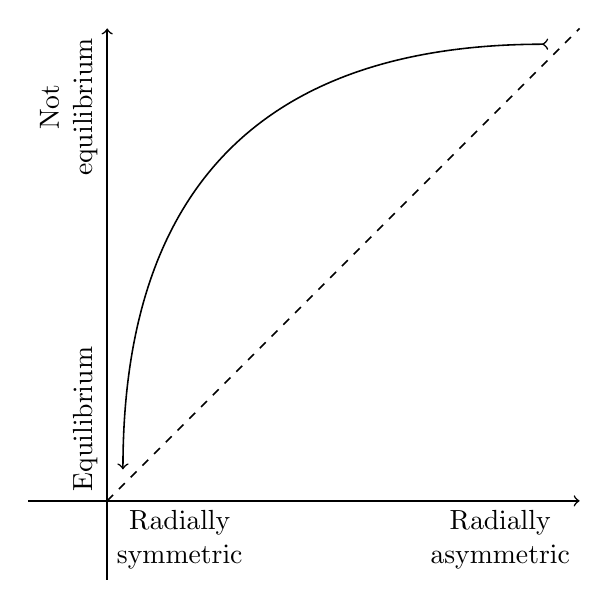
\begin{tikzpicture}
    \draw[line width=0.02cm, <-<] (0.2,0.4) .. controls (0.2,4) and (2,5.8) .. (5.6,5.8);
    \draw[line width=0.02cm, dashed] (0,0) -- (6,6);
    \draw[line width=0.02cm, ->] (-1,0) -- (6,0);
    \draw[line width=0.02cm, ->] (0,-1) -- (0,6);
    \node[below right,align=center] at (0,0) {Radially\\symmetric};
    \node[below left,align=center] at (6,0) {Radially\\asymmetric};
    \begin{scope}[cm={0,1,-1,0,(0,0)}, every node/.style={transform shape}]
        \node[above right,align=center] at (0,0) {Equilibrium};
        \node[above left,align=center] at (6,0) {Not\\equilibrium};
    \end{scope}
\end{tikzpicture}
\caption{The expected path of a solution to \eqref{eqn:boltzmann-sphom} charted on a qualitative plane
measuring distance to equilibrium and degree of radial symmetry. Note that since equilibrium solutions are
radially symmetric, the space of allowable solutions forms an open-ended triangle.}
\label{fig:offset-heuristic}
\end{figure}

\section{Numerical results} \label{sec:numerical-fou}

We study the accuracy of Fourier spectral discretizations numerically for various
situations, some of which are ``friendly'' to the hyperbolic cross, whereas others
are not. To summarize, the three methods we have used are
\begin{itemize}
    \item FF: The full grid Fourier approximation, see Section~\ref{sec:hyper}.
    \item HC: The ``raw'' hyperbolic cross method, see Section~\ref{sec:hyper}.
    \item OM: The offset method with hyperbolic cross, see Section~\ref{sec:offs}.
\end{itemize}

In Section~\ref{sec:verify} we apply the FF and HC methods to the BKW solution
to verify correctness, and to show that the hyperbolic cross does indeed do a
poor job of resolving Maxwellians. We also show numerical evidence of the
monotonic increase of entropy and its convergence to the theoretical maximum,
given by the entropy of the equilibrium distribution.

In Section~\ref{sec:crossed} we apply the method to a highly anisotropic
solution where the hyperbolic cross performs much better.

In Section~\ref{sec:relax} we give numerical evidence that the
relaxation to equilibrium is indeed exponential in time, as demonstrated by
\cite{Gressman2011gcs}.

In Section~\ref{sec:decay} we provide some numerical evidence for the exponential
decay of $f_R$ stated in Conjecture~\ref{ass:decay}, which allowed us to prove the
error estimates in Section~\ref{sec:err-trunc}.

Finally, in Section~\ref{sec:aliasing} we investigate the effect the choice of
the ratio $\kappa=\frac{R}{L}$ can have on the numerical solution.

In each case, we worked with $d=2$, and $\lambda=0$ (which is the Maxwellian
collision kernel). All timestepping was done using an explicit
4\textsuperscript{th} order Runge-Kutta method. The kernel modes were computed
with sufficiently high order Gaussian quadrature.

\subsection{Verification (BKW)} \label{sec:verify}

As a verification of correctness, one can use the only known analytic
non-equilibrium solution to the Boltzmann equation—the rotationally symmetric BKW
solution \cite{Bobylev1975esb,Krook1977esb,Tourenne1983ebs,Ernst1984esn}. It takes the form
\begin{equation} \label{eqn:bkw}
    f(t,v) = (2\pi s)^{-d/2} \exp\left(-\frac{|\Bv|^2}{2s}\right)
            \left(1-\frac{1-s}{2s} \left(d-\frac{|\Bv|^2}{s}\right)\right)
\end{equation}
where 
\[
    s = s(t) = 1 - e^{-\zeta(t+t_0)},
\]
and $B=\text{const.}$ (also called the {\em Maxwellian} kernel). Here,
$\zeta$ is a parameter given in terms of $B$, and for $d=2$ we find
$B=\frac{1}{2\pi}$ and $\zeta = \frac{1}{8}$. Finally, $t_0$ is any
reasonable starting time so that $f(t,\Bv)\geq0$ everywhere. We will use a
$t_0$ determined by $s(0) = \frac{1}{2}$, which gives the initial distribution
\[
    f_0(\Bv) = \frac{1}{\pi}|\Bv|^2e^{-|\Bv|^2}.
\]
This can be scaled to ensure that it meets the conditions of Proposition~\ref{prop:trunc} to a sufficient
degree. We use $L=3\pi$ and a scaling in $\Bv$ with factor $5$ (i.e. $f_0(5\Bv)$). This is a relatively
large value, which eliminates aliasing to machine precision level, but which also makes the Fourier series
approximation quite poor. For gases having narrow support in $\Bv$-space and wide support in $\Bk$-space.

\begin{figure}
    \centering
    \subfloat[Relative error w.r.t. time for 
               about $3100$ degrees of freedom.]{
        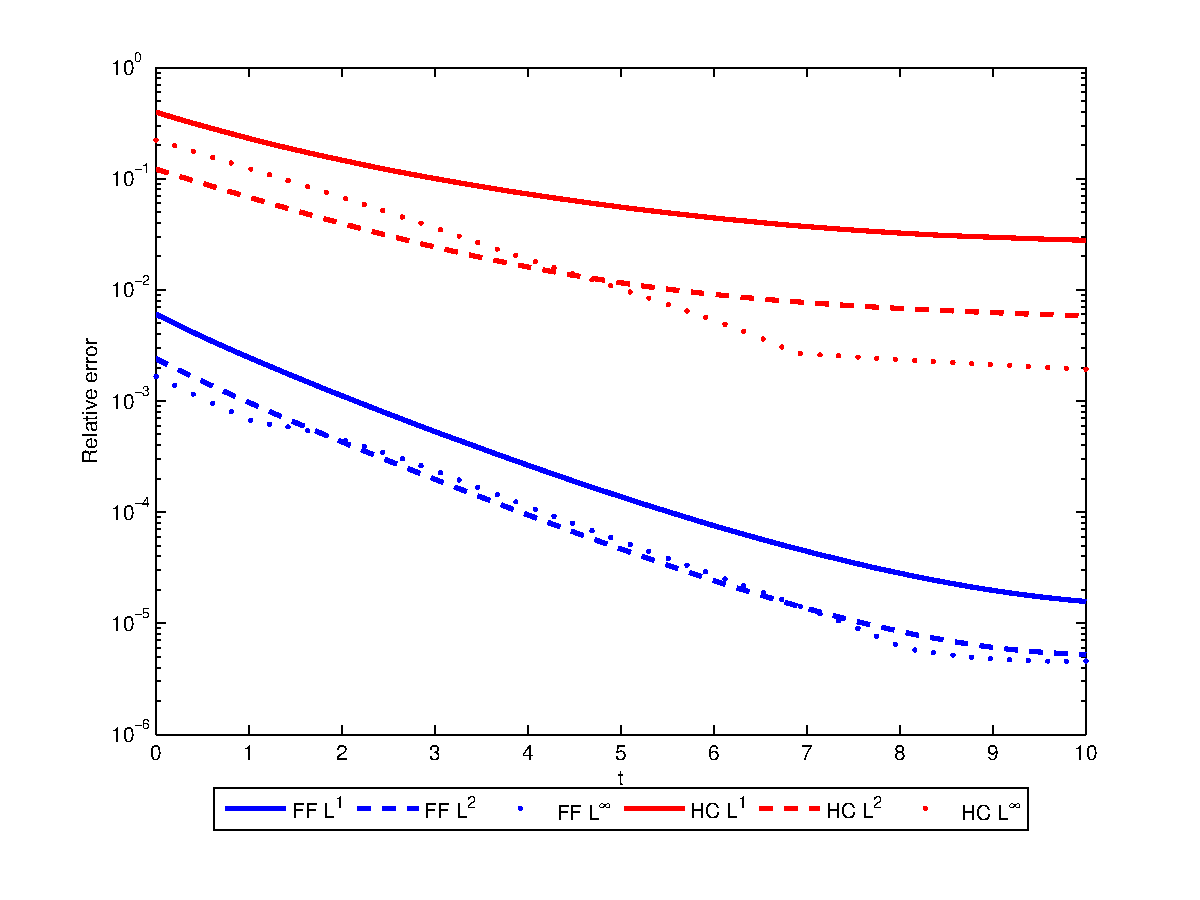
\includegraphics[width=11cm, height=7cm]{figs/hcboltz/bkwtime}
        \label{fig:bkw:time}
    }\\
    \subfloat[Relative error w.r.t. degrees of freedom at time $t=5.1$.]{
        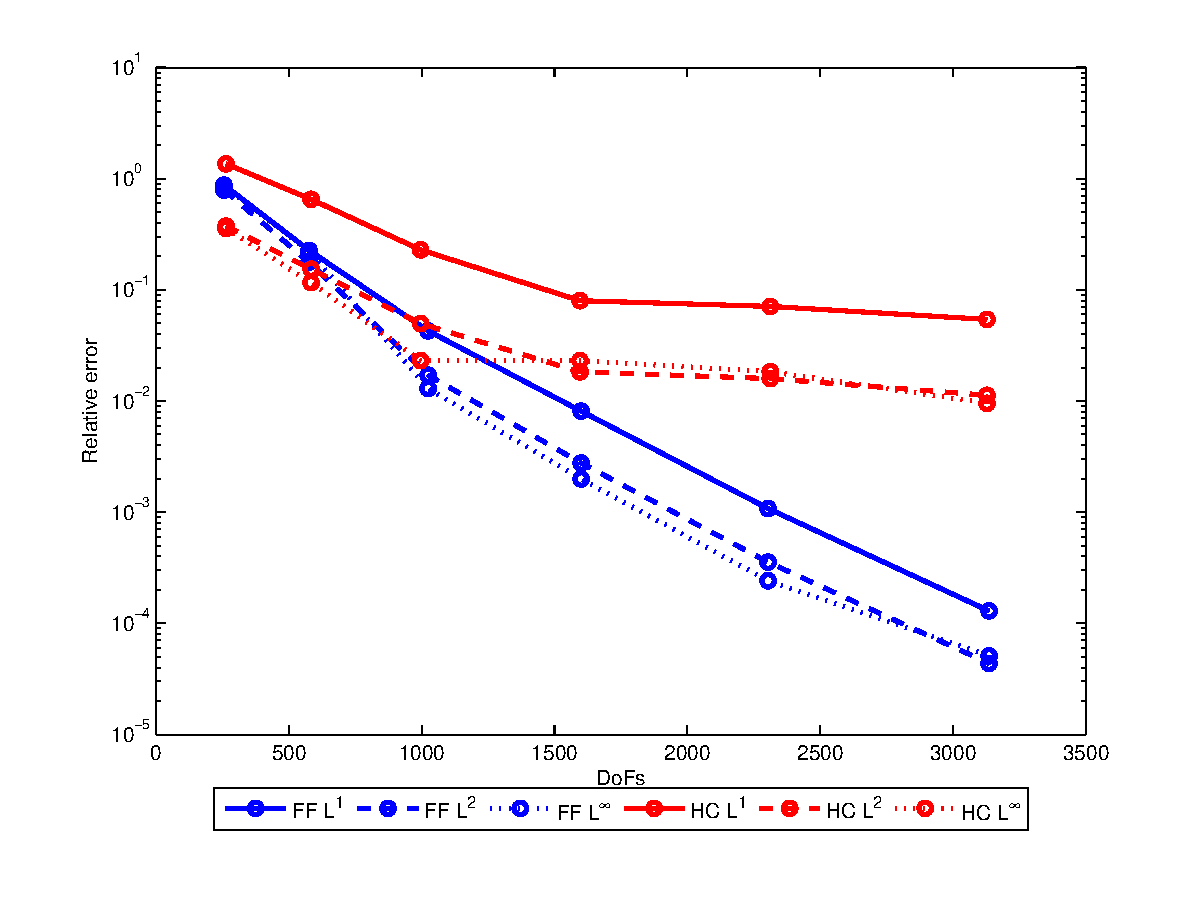
\includegraphics[width=11cm, height=7cm]{figs/hcboltz/bkw5-1}
        \label{fig:bkw:5.1}
    }
    \caption{Relative errors for the BKW solution for the full grid and hyperbolic cross methods, in $L^1$-,
    $L^2$- and $L^\infty$-norms. For timestepping, we used a fixed-timestep explicit 4\textsuperscript{th}
    order Runge-Kutta method with timestep $10^{-2}$. See Section~\vref{sec:verify} for details.}
    \label{fig:bkw} 
\end{figure}

Figure~\vref{fig:bkw} shows the results for this experiment. Note the poor approximation properties due to the
very narrow support of $f_0$, as well as the poor performance of the hyperbolic cross, due to the rotational
symmetry.  Note also how inaccurate initial data can still yield accurate long-term solutions. The solutions
themselves are shown in Figure~\vref{fig:bkw:sols}. Finally, Figure~\vref{fig:entropy} shows, for $N=56$, how
the entropy of the solution, 
\[ -\int_{\cD_L} f(\Bv)\log f(\Bv) \dd \Bv \] 
converges to the theoretical maximum as given by the equilibrium distribution.

\begin{figure}
    \centering
    \subfloat[Initial distribution.]{
        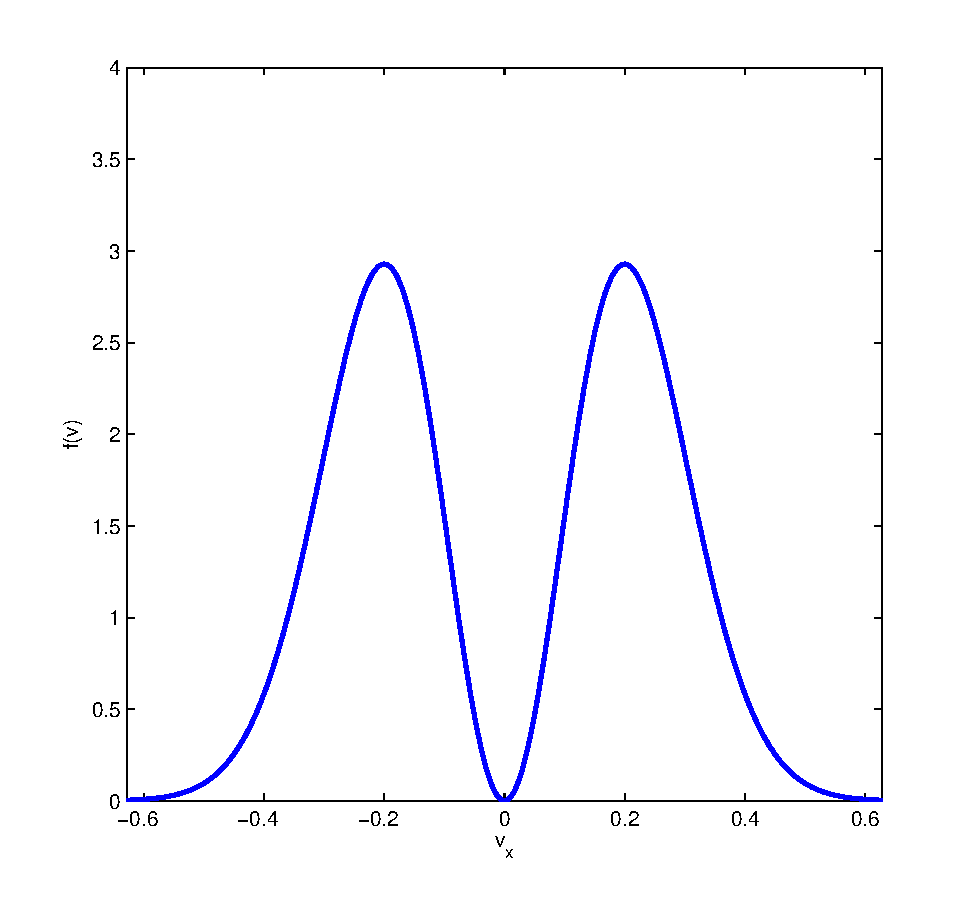
\includegraphics[width=6.45cm,height=6cm]{figs/hcboltz/bkwstart}
        \label{fig:bkw:start}
    }
    \subfloat[Equilibrium.]{
        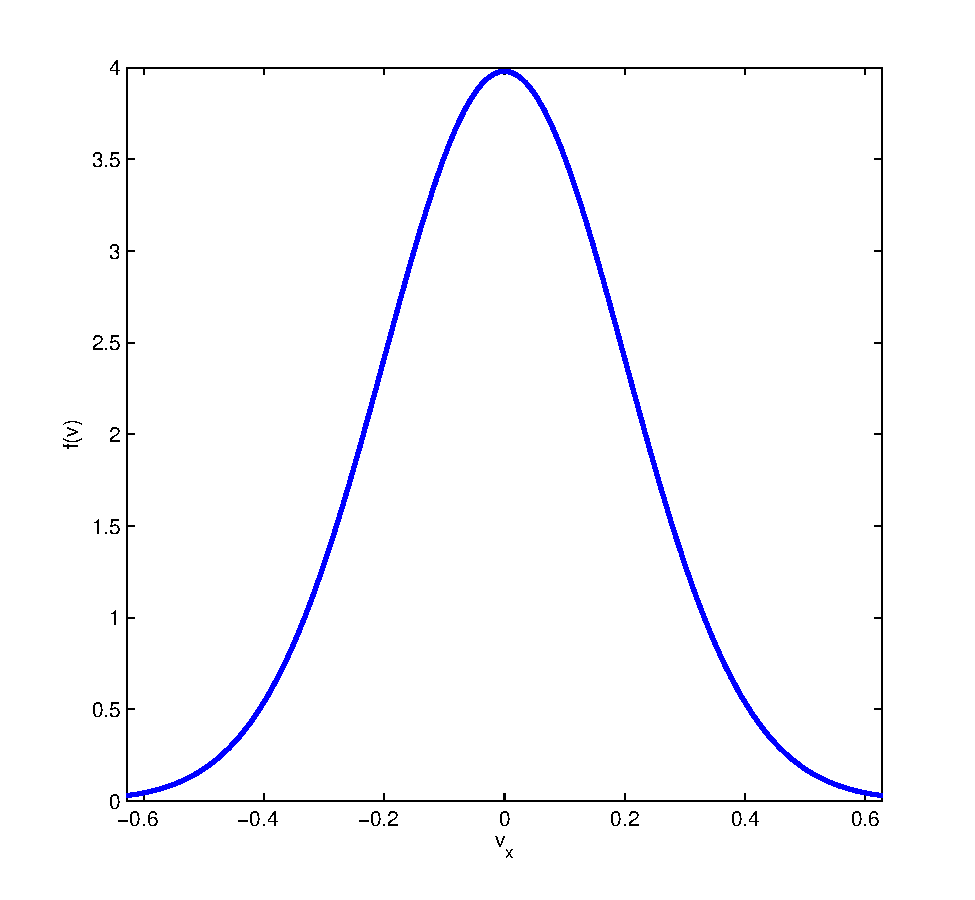
\includegraphics[width=6.45cm,height=6cm]{figs/hcboltz/bkweq}
        \label{fig:bkw:eq}
    }
    \caption{Cross-section plots of the BKW solution. Rotational symmetry applies. See
    Section~\vref{sec:verify} for details.}
    \label{fig:bkw:sols}
\end{figure}

\begin{figure}
    \centering
    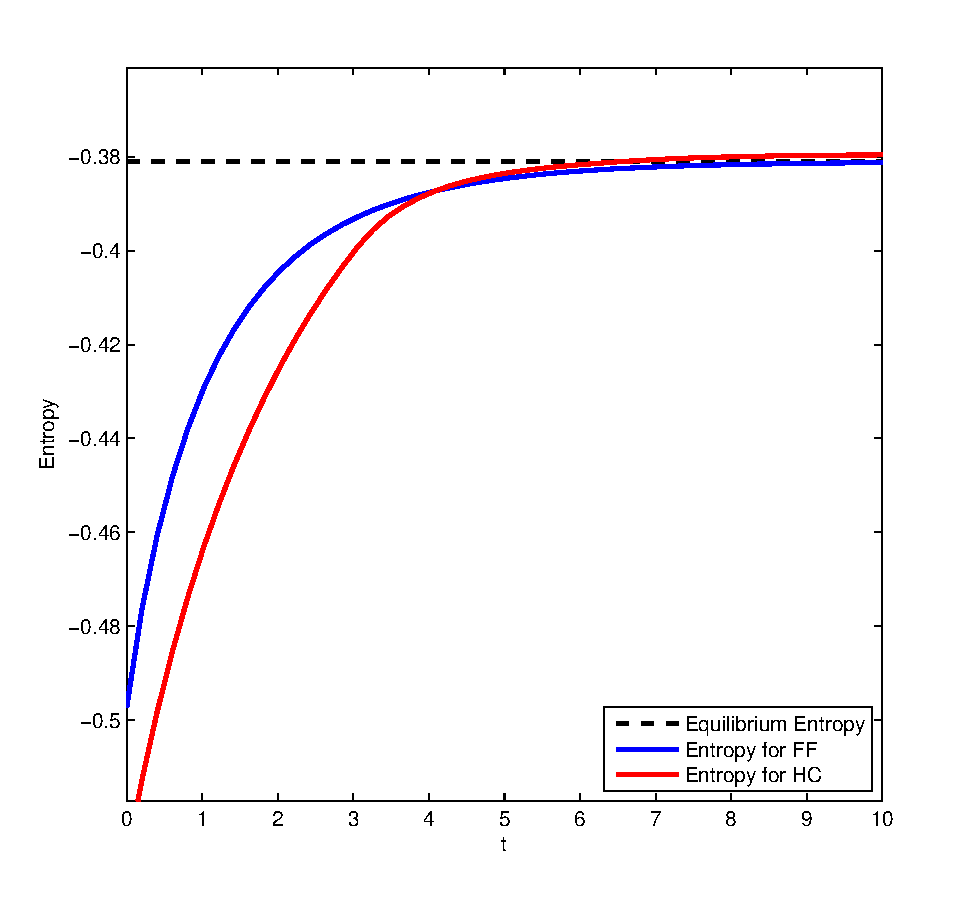
\includegraphics[width=7cm]{figs/hcboltz/entropy}
    \caption{Convergence of entropy for $\AFF(56)$ (correct) and $\cA_0(234)$ (incorrect) for the BKW
    solution. See Section~\vref{sec:verify} for details.}
    \label{fig:entropy}
\end{figure}

\clearpage

\subsection{Crossed streams} \label{sec:crossed}

This is an example of a case where the hyperbolic cross approximation works
very well. The initial condition is 
\[
    f_0(\Bv) = \left[(1+\sin(sv_x))e^{-sv_x^2} + 
            (1+\sin(sv_y))e^{-sv_y^2}\right] e^{-2|\Bv|^2}.
\]
There parameter $s>0$ can be tweaked to make $f_0$ more or less isotropic.  For
our experiment we have used $s=10$, and a hyperbolic cross with standard
fatness $T=0$.  We computed the solution over four time units, with an explicit
4\textsuperscript{th} order Runge-Kutta method with timestep $5\cdot10^{-3}$.

Since this is beyond the scope of known analytic solutions, we used a reference
solution computed on a full grid with $N=80$. The results for global
$L^2$-errors are shown in Figure~\vref{fig:hc1:l2}, and for observables in
Figure~\vref{fig:hc1:obs}.

In these cases, the hyperbolic cross can be seen to outperform the full grid
method, although the latter catches up over time and eventually wins out as the
solution approaches equilibrium, see Figure~\vref{fig:hc1:l2:time}.

\begin{figure}
    \centering
    \subfloat[Relative error at time $t=0$.]{
        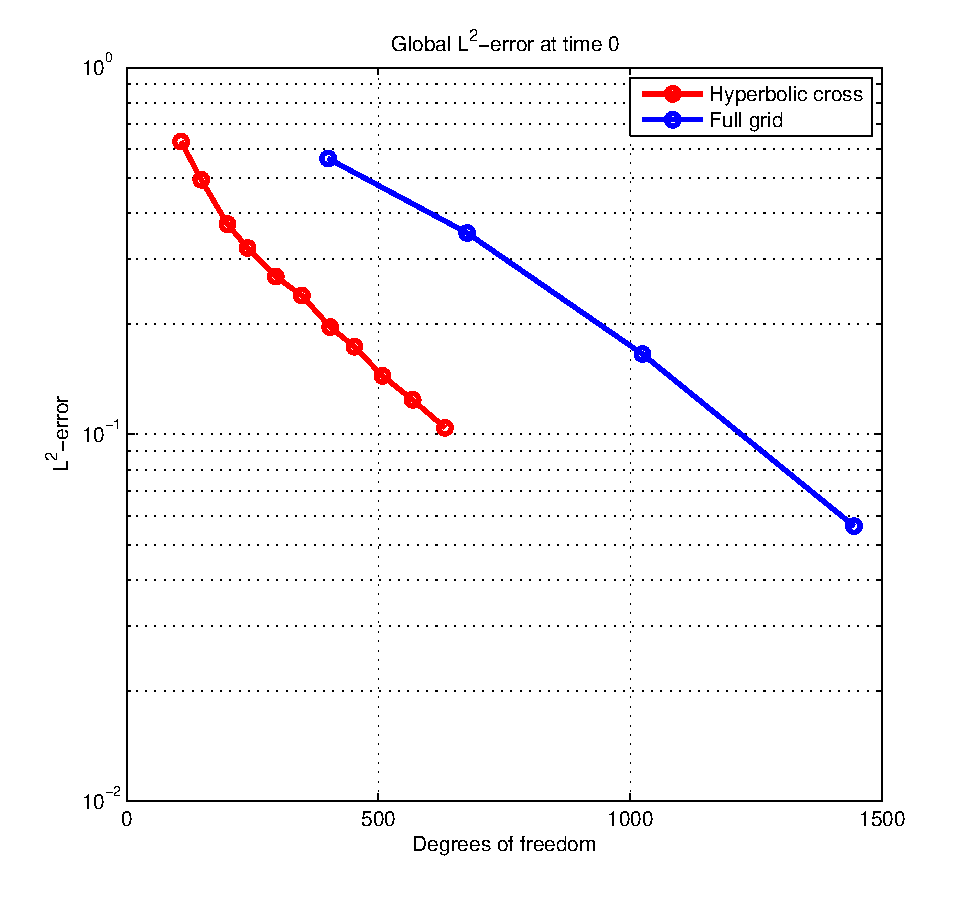
\includegraphics[width=6.8cm]{figs/hcboltz/hc1-l2-1}
        \label{fig:hc1:l2:1}
    }
    \hspace{-1.5cm}
    \subfloat[Relative error at time $t=0.96$.]{
        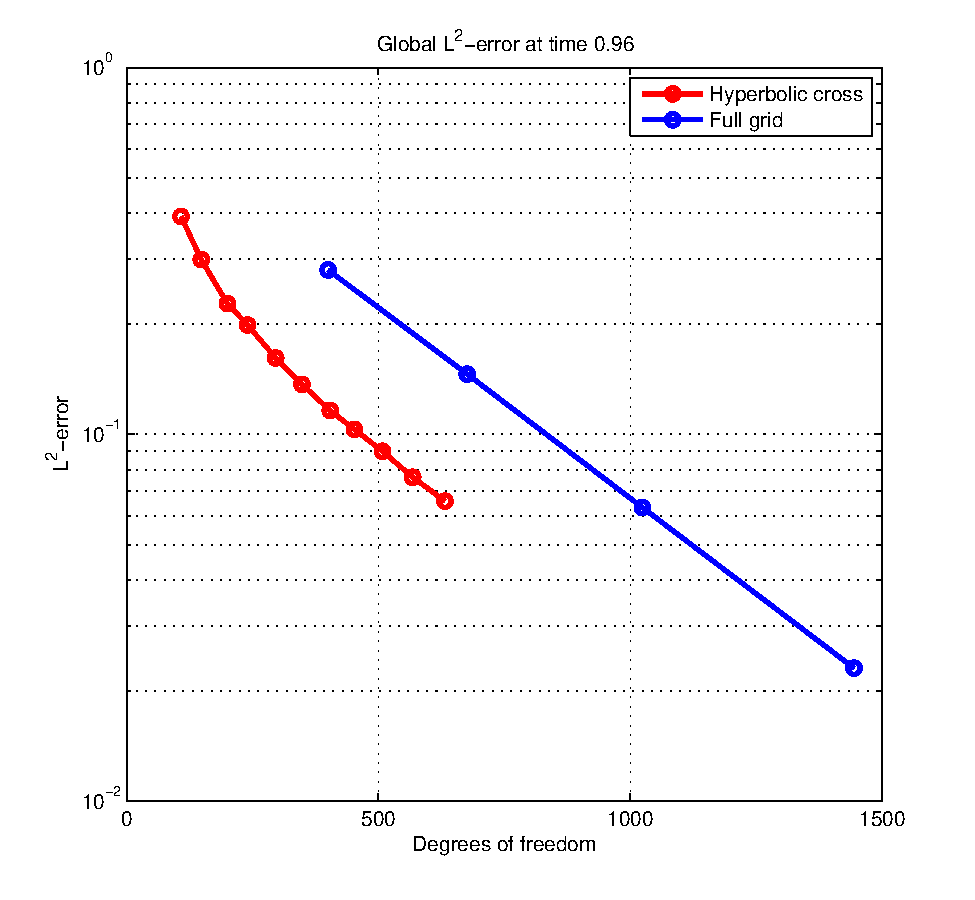
\includegraphics[width=6.8cm]{figs/hcboltz/hc1-l2-2}
        \label{fig:hc1:l2:2}
    }
    \\
    \subfloat[Relative error at time $t=2$.]{
        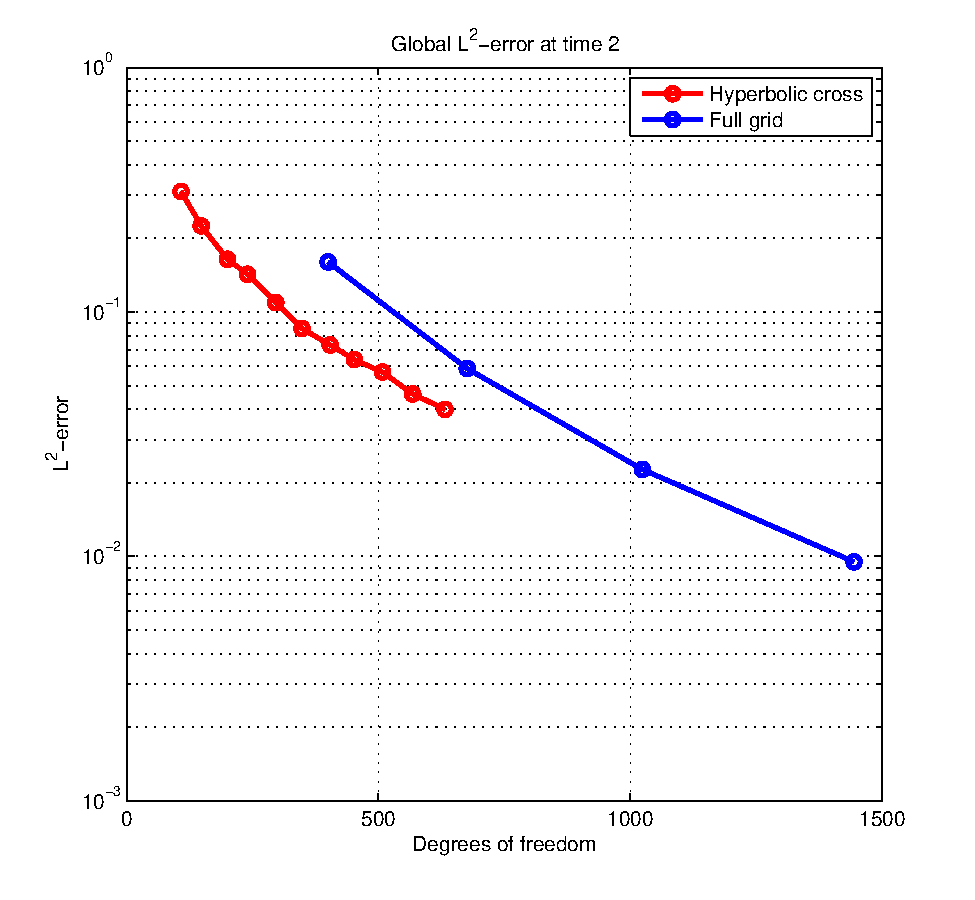
\includegraphics[width=6.8cm]{figs/hcboltz/hc1-l2-3}
        \label{fig:hc1:l2:3}
    }
    \hspace{-1.5cm}
    \subfloat[Relative error over time for $676$ and $632$ degrees of freedom, respectively.]{
        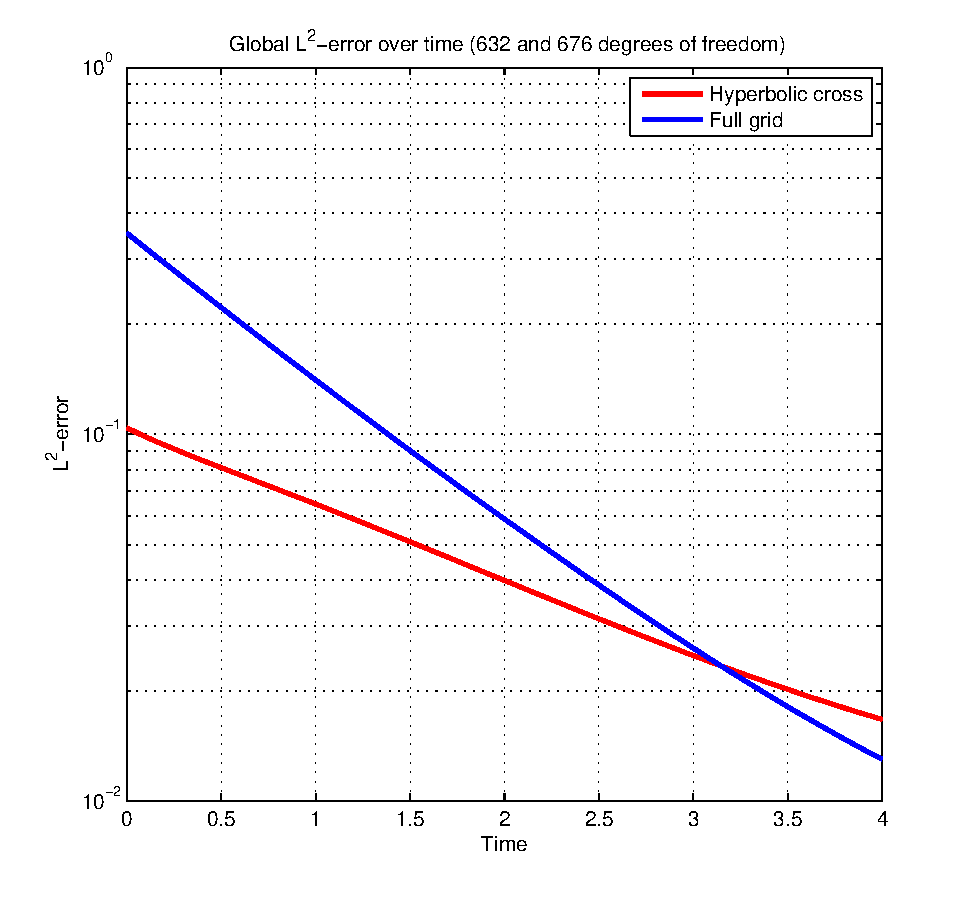
\includegraphics[width=6.8cm]{figs/hcboltz/hc1-l2-time}
        \label{fig:hc1:l2:time}
    }
    \caption{Relative $L^2$-errors for the crossed streams experiment. See Section~\vref{sec:crossed} for
    details.}
    \label{fig:hc1:l2}
\end{figure}

\begin{figure}
    \centering
    \subfloat[Error in observables at time $t=0$.]{
        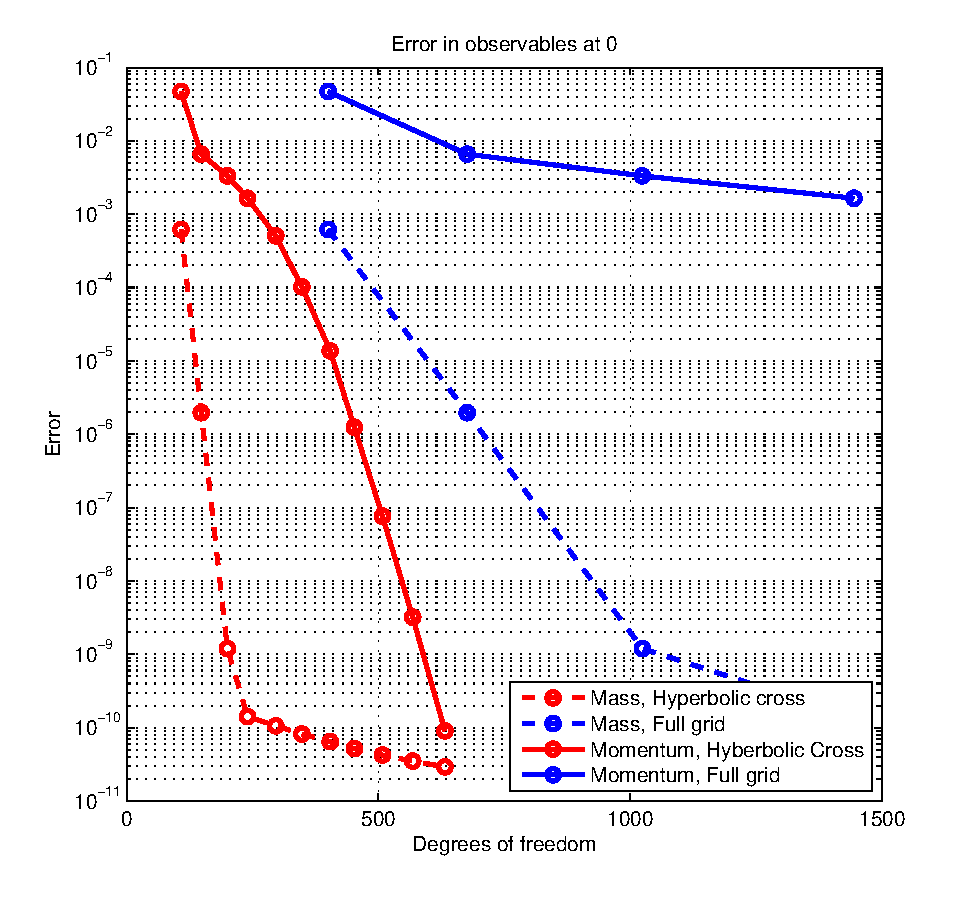
\includegraphics[width=7cm]{figs/hcboltz/hc1-obs-1}
        \label{fig:hc1:obs:1}
    }
    \subfloat[Error in observables at time $t=2$.]{
        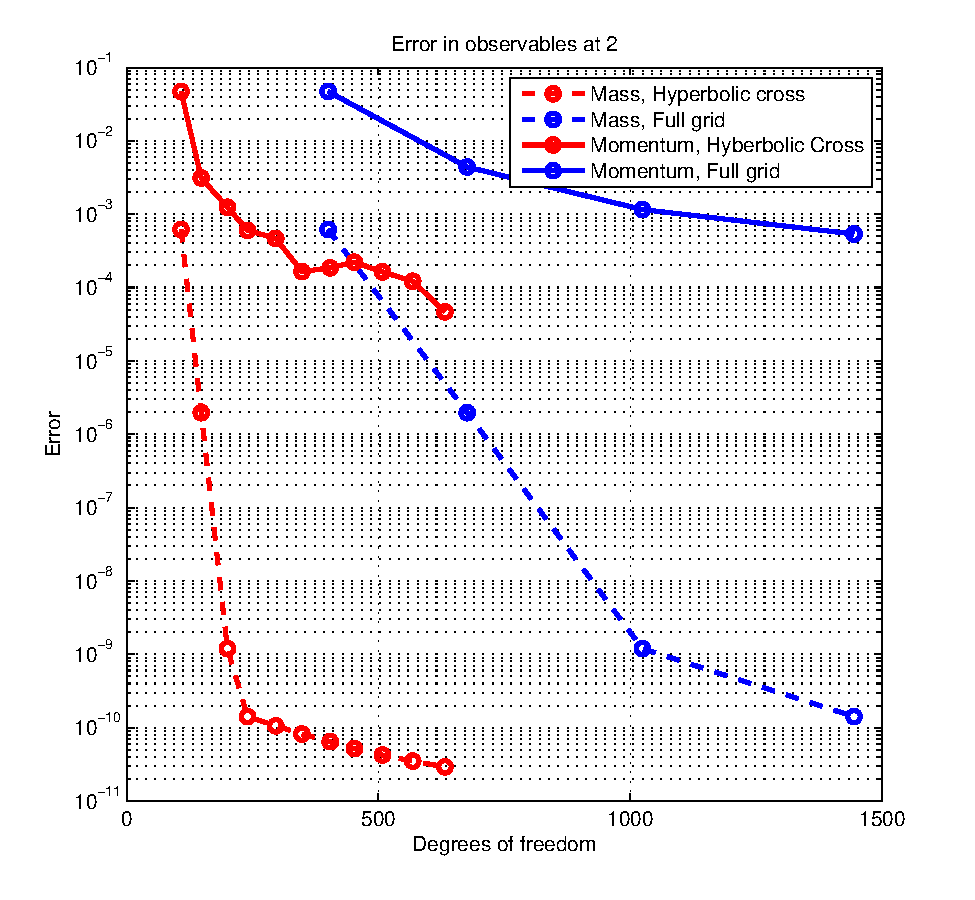
\includegraphics[width=7cm]{figs/hcboltz/hc1-obs-3}
        \label{fig:hc1:obs:3}
    }
    \caption{Errors in observables for the crossed streams experiment. See Section~\vref{sec:crossed} for
    details.}
    \label{fig:hc1:obs}
\end{figure}

\begin{figure}
    \centering
    \subfloat[Initial distribution.]{
        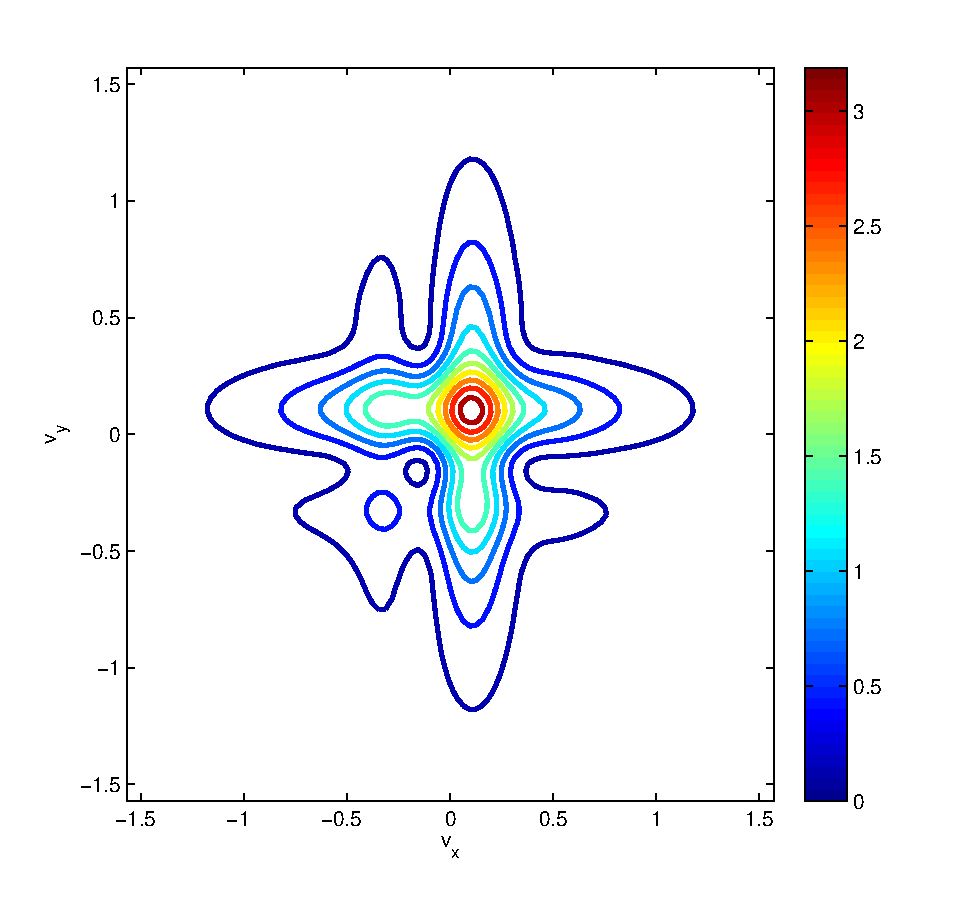
\includegraphics[width=6.45cm,height=5cm]{figs/hcboltz/crossed-1}
        \label{fig:hc1:start}
    }
    \subfloat[Solution at time $t=2$.]{
        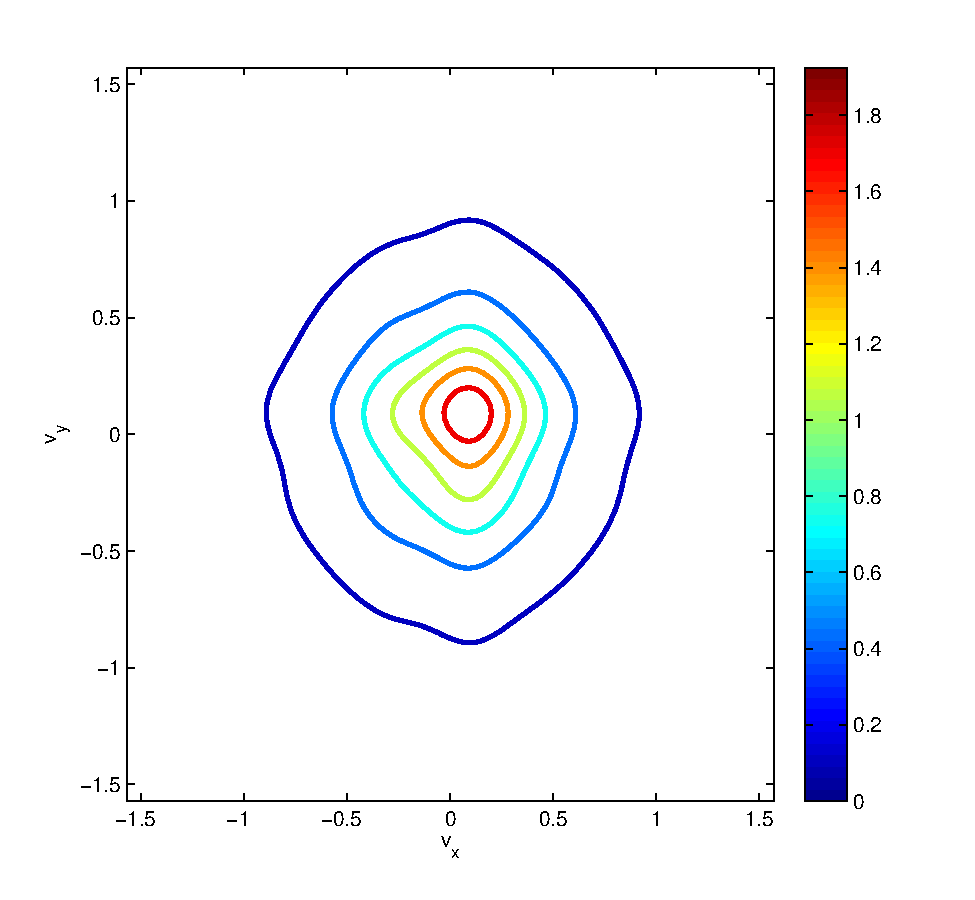
\includegraphics[width=6.45cm,height=5cm]{figs/hcboltz/crossed-3}
        \label{fig:hc1:eq}
    }
    \caption{The crossed streams solution. See Section~\vref{sec:crossed} for details.}
    \label{fig:hc1:sols}
\end{figure}

\subsection{Relaxation to equilibrium} \label{sec:relax}

This is an example of the offset method from Section~\ref{sec:offs}, using the initial distribution
\[
    f_0(\Bv) = e^{-2|\Bv|^2} + \epsilon\left(e^{-sv_x^2-v_y^2} + 
            e^{-v_x^2-sv_y^2}\right),
\]
where again the parameter $s>1$ controls the anisotropy of $f_{0}$, and
$\epsilon>0$ represents the fact that $f_0$ is a minor perturbation from
equilibrium.\footnote{Note that equilibrium is {\em not} $e^{-2|\Bv|^2}$ ---
the perturbation adds both mass density and temperature.}

Using $s=7$ and $\epsilon=10^{-2}$, we have plotted $\|f^p\|$ from \eqref{eq:fp}
versus time for three different norms in Figure~\vref{fig:relaxation}. The
convergence halts at $\|f^p\|\approx10^{-5}$ due to truncation error in $\Bv$ for
all norms, but prior to this, exhibits behavior in accordance with
\cite{Gressman2011gcs}.

\begin{figure}
    \centering
    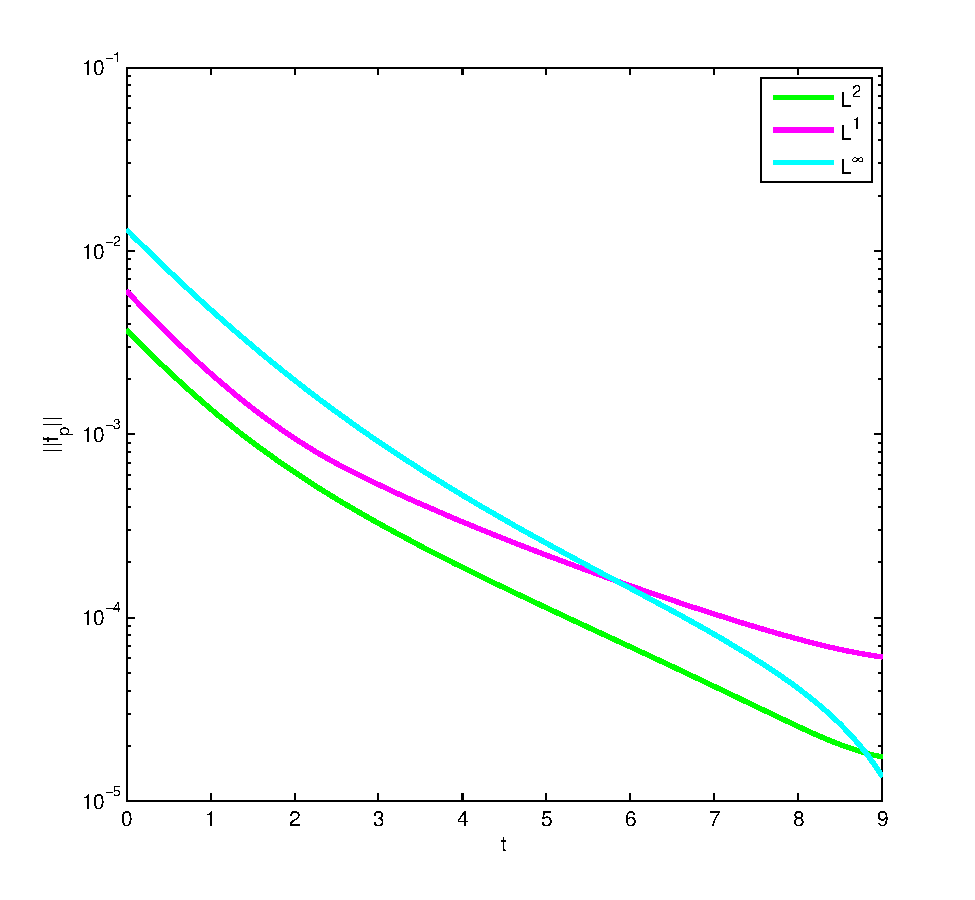
\includegraphics[width=10cm]{figs/hcboltz/ds-pertnorms}
    \caption{Relaxation to equilibrium (see Section~\vref{sec:relax} for details):
      norms of the perturbation of the offset method versus time.} 
    \label{fig:relaxation}
\end{figure}

\subsection{Exponential decay of the numerical solution} \label{sec:decay}

We will here provide some numerical evidence that a certain exponential decay
can be expected to hold for the numerical solution using both $\AFF(N)$ and
$\cA_0(N)$ with some unspecified dependence $N=N(L)$. The decay we are after is
the existence of some $C$ independent of $L$ so that
\[
    \|f_{\cA(L)} \mu_a^{-1}\|_{L^2(\cD_L)} \leq C L^{\nicefrac{d}{2}}
\]
where $\mu_a$ is a Maxwellian with some decay rate $a$,
\[
    \mu_a(\Bv) = e^{-a|\Bv|^2}.
\]
This might go some way towards justifying Conjecture~\ref{ass:decay}. Note that the dependence on $L$ on the
right hand side is necessary in the limit $f_{\cA(L)} \to \mu_a$.

Table~\vref{tbl:numbers} shows these norms for various $N$ and $L$. For the $L$
chosen, a stable result of $\|f_{\cA(L)} \mu_a^{-1}\|_{L^2(\cD_L)}
\approx 1.3$ was achieved with relatively modest numbers of degrees of freedom.

A test with large values of $L$ would be difficult to perform with the current 
implementation, as the exponential weight at the boundaries of $\cD_L$ is much
larger than machine precision, artificially inflating the norms.

\begin{table}
\centering
\subfloat[$\AFF$]{
    \def\arraystretch{1.2}
    \begin{tabular}{c|c c c}
    $N$ & $L=0.5\pi$ & $L=0.75\pi$ & $L=\pi$ \\
    \hline 12 & 1.25 & 1.25 & 299  \\
    16 & 1.25 & 1.25 & 1.74 \\
    20 & 1.25 & 1.25 & 1.28 \\
    24 & 1.25 & 1.25 & 1.28 \\
    28 & 1.25 & 1.25 & 1.28 \\
    \end{tabular}
} \\
\subfloat[$\cA_0$]{
    \def\arraystretch{1.2}
    \begin{tabular}{c|c c c}
    $N$ & $L=0.5\pi$ & $L=0.75\pi$ & $L=\pi$ \\
    \hline 50 & 1.25 & 1.30 & $5.25\cdot10^4$ \\
    70 & 1.25 & 1.25 & $5.67\cdot10^3$ \\
    90 & 1.25 & 1.25 & $1.15\cdot10^3$ \\
    110 & 1.25 & 1.25 & 193 \\
    130 & 1.25 & 1.25 & 10.5 \\
    150 & 1.25 & 1.25 & 1.99 \\
    170 & 1.25 & 1.25 & 1.29 \\
    190 & 1.25 & 1.25 & 1.28 \\
    \end{tabular}
}
\caption{
    Numerical evidence for the exponential decay of $f_\cA$ (see Section~\vref{sec:decay} for details).
    The table shows $\sup_t\|f_\cA \mu_a^{-1}\|_{L^2(\cD_L)}$ for various $N$ and $L$. The test case
    was the crossed streams setup from Section~\vref{sec:crossed}, and integrated until $T=10$.
}
\label{tbl:numbers}
\end{table}

\subsection{Aliasing and anti-aliasing} \label{sec:aliasing}

The ratio $\kappa=\nicefrac{R}{L}$ can be adjusted to control aliasing between
different periods of the numerical solution. A small choice of $\kappa$ will
avoid aliasing for several timesteps, while a large choice will allow all
possible collisions to be treated in a single timestep.

The following Figures show the evolution for the BKW solution using $N=32$
degrees of freedom in each direction using a full Fourier grid over the time
interval $[0,10]$.

The initial and final distribution for $\kappa=\frac{2}{3+\sqrt{2}}\approx
0.45$ is shown in Figure~\vref{fig:r:normal}. It is clear that the solution
maintains its equilibrium very well due to the low aliasing.

\begin{figure}
    \centering
    \subfloat[Initial distribution.]{
        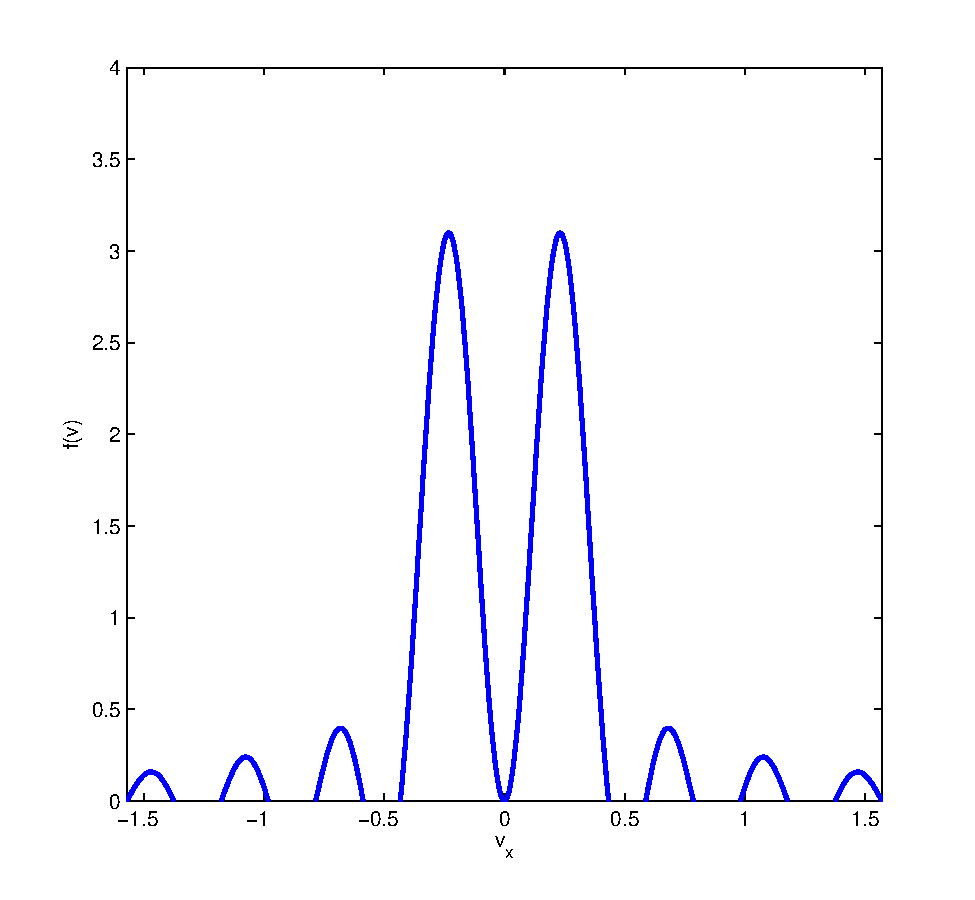
\includegraphics[width=6.8cm]{figs/hcboltz/bkw-r-normal-init}
        \label{fig:r:normal:init}
    }
    \subfloat[Solution at time $t=40$.]{
        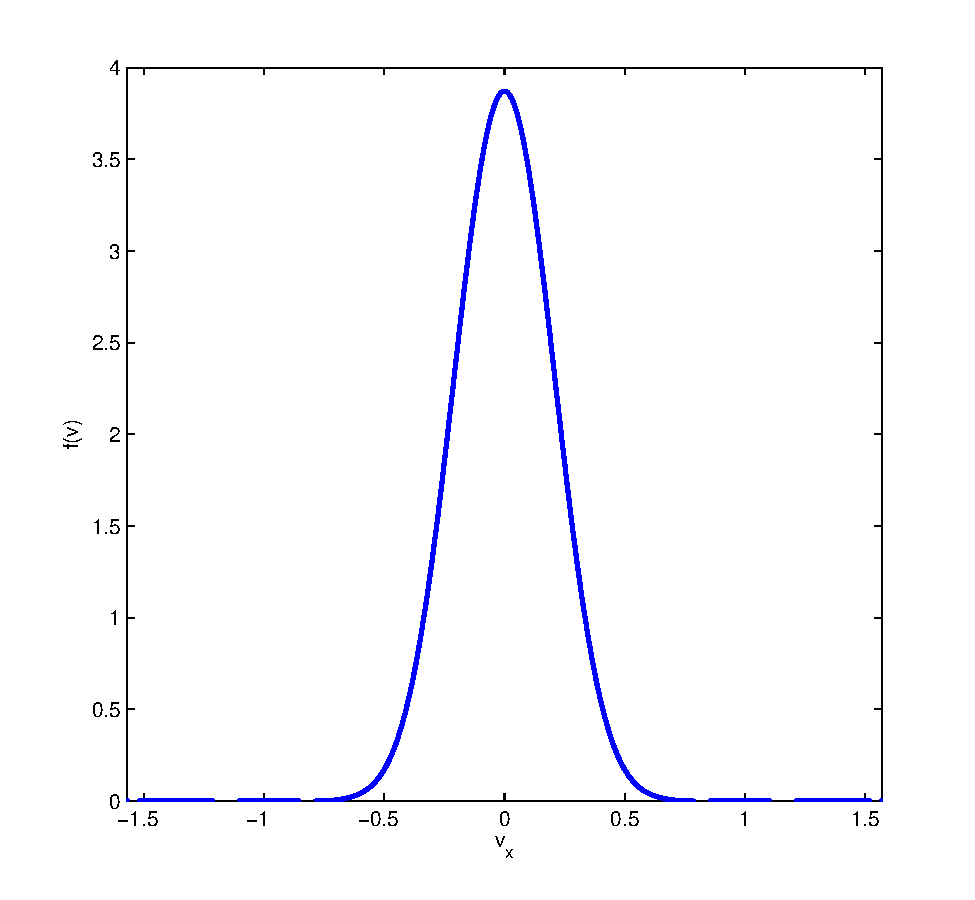
\includegraphics[width=6.8cm]{figs/hcboltz/bkw-r-normal-end}
        \label{fig:r:normal:end}
    }
    \caption{Initial and final discrete solution for the BKW experiment using $\kappa\approx0.45$. Compare to
    Figure~\vref{fig:r:sqrt2}. Note the $y$-axis scales.}
    \label{fig:r:normal}
\end{figure}

\begin{figure}
    \centering
    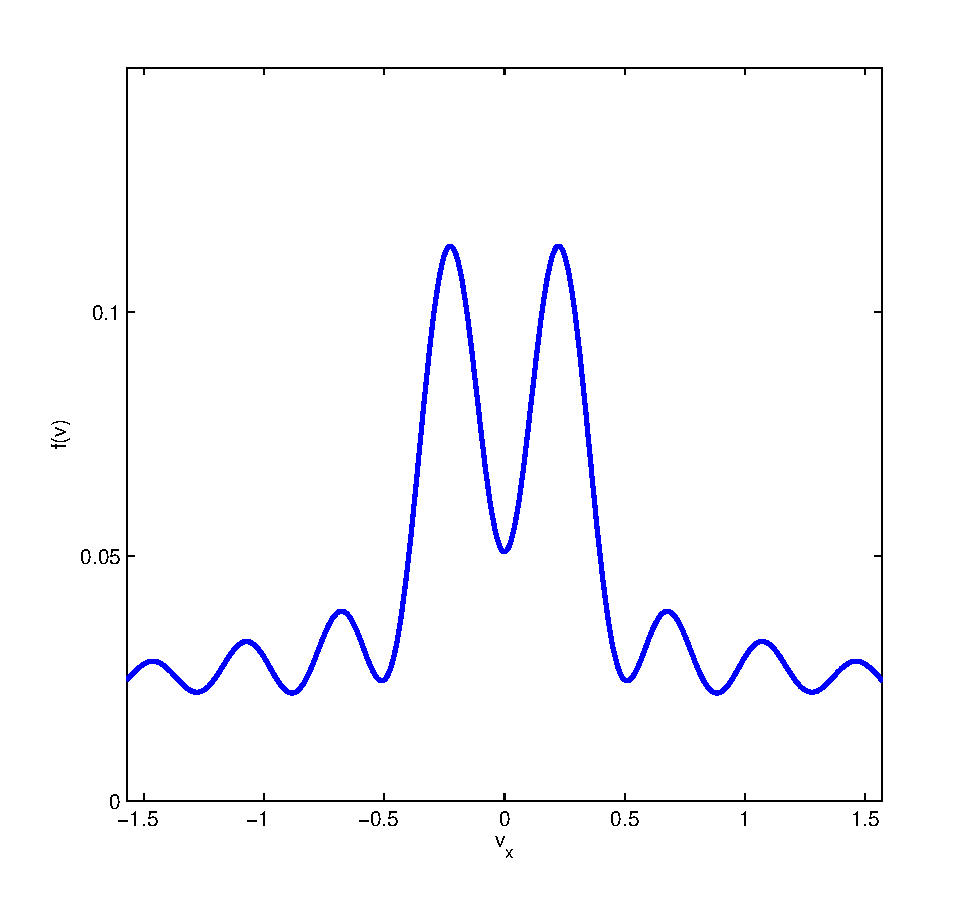
\includegraphics[width=6.8cm]{figs/hcboltz/bkw-r-sqrt2-end}
    \caption{Solution at time $t=0.6$ for the BKW experiment using $\kappa=\sqrt{2}$. Compare to
    Figure~\ref{fig:r:normal}. Note the $y$-axis scales.}
    \label{fig:r:sqrt2}
\end{figure}

In \cite{Filbet2011asm}, time-global consistency and convergence is shown under
various assumptions, one of which is $\kappa\geq\sqrt{2}$. The distribution for
this scheme at $t=0.6$ is shown in Figure~\vref{fig:r:sqrt2}. This time is well
before equilibrium is reached, and the effect of significant aliasing can be
seen. The solution is clearly nonphysical.

Figure~\vref{fig:testr} shows the time-evolution of the $L^2$-error for the BKW
solution for various $\kappa$, ranging from $0.45$ to $\sqrt{2}$. For long
times, the error will always tend toward $0.9935$, which happens to be the
$L^2$-norm between the physical equilibrium solution (the Maxwellian), and the
numerical equilibrium solution (a constant function). We observe that for large
$\kappa$, the numerical solution collapses to a constant very rapidly, and for
smaller $\kappa$, the solution remains qualitatively correct for much longer
times.

\begin{figure}
    \centering
    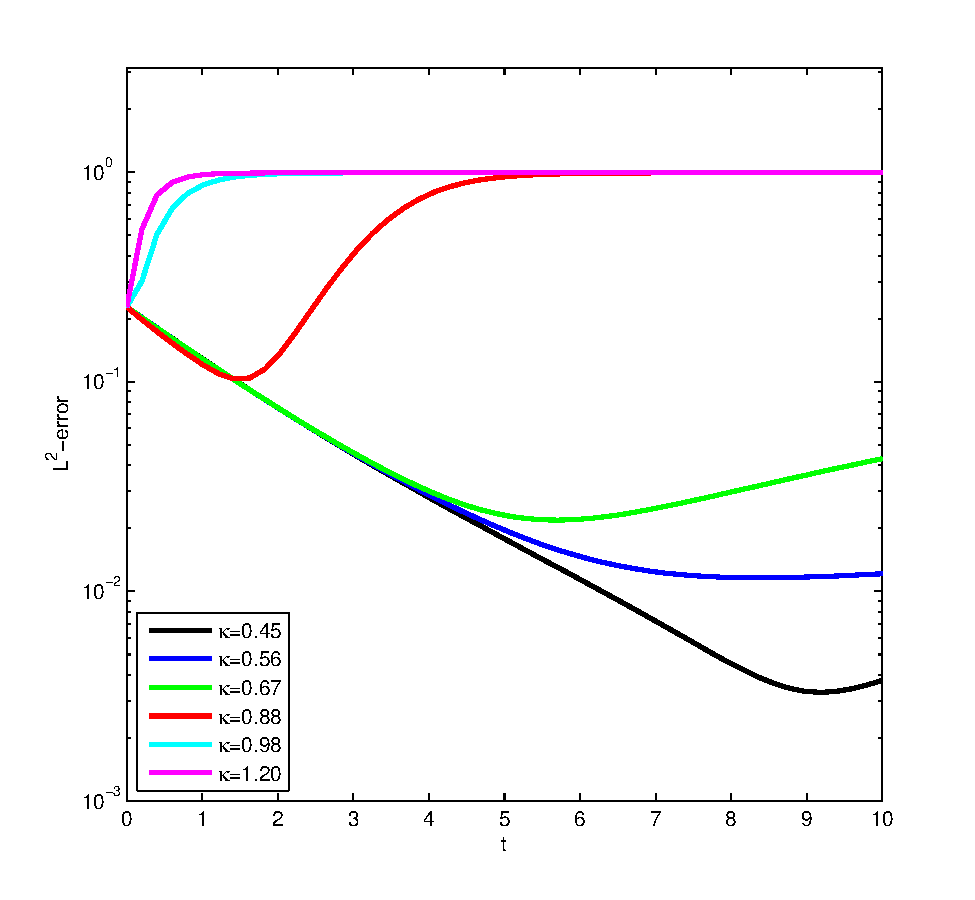
\includegraphics[width=10cm]{figs/hcboltz/testr}
    \caption{$L^2$-error versus time for the BKW solution at various $\kappa$. See the discussion in
    Section~\vref{sec:aliasing} for details.}
    \label{fig:testr}
\end{figure}
